\documentclass[9pt,t,aspectratio=1610]{beamer} 

\usepackage[utf8]{inputenc}
\usepackage[T1]{fontenc}
\usepackage{svg}
\usepackage{amsmath}
\usepackage{bbm}            % mathbb vs mathds
% \usepackage{amsthm,amssymb}
% \usepackage[numbers]{natbib}
\usepackage{bibentry}  % bibtex elements into text
% \usepackage{animate}

\usepackage{biolinum} % new font
\usepackage{booktabs}  % for \specialrule
\usepackage{pifont}  % symbols (like \ding)
\usepackage{tcolorbox}


% --------------------------------------------------------------------------------------------------
% Template
% --------------------------------------------------------------------------------------------------
% \usetheme{default}
% \usecolortheme{default}

% My colors
% \definecolor{myblue}{RGB}{31, 119, 180}
% \definecolor{myorange}{RGB}{230, 107, 0}
% \definecolor{mygreen}{RGB}{0, 135, 30}

\definecolor{myblue}{RGB}{31, 119, 180}
\definecolor{myorange}{RGB}{245, 117, 4}
\definecolor{mygreen}{RGB}{34, 150, 34}

\usecolortheme[named=myblue]{structure}
\setbeamercolor{itemize subitem}{fg=myorange}
\setbeamercolor{section in head/foot}{fg=white, bg=myblue}
\setbeamercolor{subsection in head/foot}{fg=white, bg=myblue}
\setbeamercolor{section in sidebar}{fg=black, bg=myblue}
\setbeamercolor{subsection in sidebar}{fg=black, bg=myblue}
\setbeamercolor{sidebar}{bg=myblue}

\setbeamertemplate{frametitle}[default][center]
\setbeamertemplate{navigation symbols}{}% remove navigation symbols

% ajoute les numero de slides
\addtobeamertemplate{navigation symbols}{}{%
    \usebeamerfont{footline}%
    \usebeamercolor[fg]{section title}%
    \hspace{1em}%
    \normalsize{\insertframenumber/\inserttotalframenumber}
}

% pour ne pas compter toutes les frames de biblio
\setbeamertemplate{frametitle continuation}{}

% margins
\setbeamersize{text margin left=15mm,text margin right=15mm} % left and right
\addtobeamertemplate{frametitle}{\vspace*{2mm}}{\vspace*{0mm}} % top and bottom

% to have the section and subsection number in the table of contents
\setbeamertemplate{section in toc}[sections numbered]
\setbeamertemplate{subsection in head/foot}[sections numbered]

% Add bar with outline
\setbeamertemplate{headline}{%
\leavevmode%
  \hbox{%
    \begin{beamercolorbox}[wd=\paperwidth,ht=0.78cm,dp=1.125ex]{section in head/foot}%
    \small
%     \insertsectionnumber
    \insertsectionnavigationhorizontal{\paperwidth}{\hskip0pt plus1filll}{\hskip0pt plus1filll}
    \footnotesize
    \insertsubsectionnavigationhorizontal{\paperwidth}{\hskip0pt plus1filll}{\hskip0pt plus1filll}
    \vfill
    \end{beamercolorbox}
  }
}

% \newlength\sidebarwd
% \setlength\sidebarwd{3.3cm}
% \setbeamersize{sidebar width left = \sidebarwd}
% \setbeamertemplate{sidebar left}{%
% \footnotesize
%     \insertsectionnavigation{0.5cm}{\vspace*{2cm}}{}
%     \insertsubsectionnavigation{2cm}{}{}
% \vfill
% }

% \setbeamercolor{background canvas}{bg=darkgray}

% \setbeamercolor{headline}{bg=gray}
% \setbeamercolor{footline}{bg=gray}
% Pour avoir des tirets dans les itemize
% \setbeamertemplate{itemize items}[$-$]

% pour faire de jolis blocs
% \usepackage{tcolorbox}
% optiions
% \tcbset{top=55mm, bottom=10mm, % marge haut et bas.
% left=0mm, right=0mm}


% --------------------------------------------------------------------------------------------------
%Information to be included in the title page:
\title{Détection d'événements à partir de capteurs sols -- application au suivi de personnes fragiles}
\subtitle{Soutenance de thèse}
\author{Ludovic Minvielle\\[0.4cm]
    Directeur: Nicolas Vayatis, Centre Borelli, ENS Paris-Saclay\\
    Co-encadrante: Mathilde Mougeot, Centre Borelli, ENS Paris-Saclay}
\institute[VFU] % (optional)
{
%     $^1$Centre Borelli, ENS Paris-Saclay\\
%     $^2$Tarkett
        Thèse industrielle entre l'ENS Paris-Saclay et Tarkett
}
\date{Mercredi 15 Juillet 2020}

\titlegraphic{
	
\includegraphics[height=6mm]{images/CMJNLogotype_Centre_Borelli_couleur_petit.png}\hspace{1em}%
	
\includegraphics[height=6mm]{images/LogoIDAML.jpg}\hspace{1em}%
    
\includegraphics[height=6mm]{images/ens-paris-saclay.png}\hspace{1em}%
	
\includegraphics[height=6mm]{images/ens-cachan.png}\hspace{1em}%
	
\includegraphics[height=6mm]{images/logo-cnrs.png}\hspace{1em}%
    
\includegraphics[height=5mm]{images/Tarkett-logo_red.jpg}\hspace{1em}%
}
% --------------------------------------------------------------------------------------------------     

% COMMANDS, SHORTUCTS
\newcommand{\myemph}[1]{\textcolor{myblue}{#1}}
\newcommand{\myemphtwo}[1]{\textcolor{myorange}{#1}}
\newcommand{\myemphthree}[1]{\textcolor{mygreen}{#1}}
\newcommand{\ratio}{0.5}
\newcommand{\algo}{{\textsc{NurseNet}}\ }
\newcommand{\subalgo}{{\small\textsc{SPN}}\ }
\newcommand{\lghline}{\arrayrulecolor{lgray}\hline}
\newcommand{\bfX}{\mathbf{X}}
\newcommand{\bfW}{\mathbf{W}}
\newcommand{\bfw}{\mathbf{w}}
\newcommand{\bfx}{\mathbf{x}}
\newcommand{\bfy}{\mathbf{y}}
\newcommand{\bfv}{\mathbf{v}}
\newcommand{\bft}{\mathbf{t}}
\newcommand{\bfu}{\mathbf{u}}
\newcommand{\bfz}{\mathbf{z}}
\newcommand{\bfs}{\mathbf{s}}
\newcommand{\bfS}{\mathbf{S}}
\newcommand{\bfd}{\mathbf{d}}
\newcommand{\bfD}{\mathbf{D}}
\newcommand{\bfI}{\mathbf{I}}
\newcommand{\bfind}{\mathbf{1}}
\newcommand{\bbmind}{\mathbbm{1}}
\newcommand\calX{\boldsymbol{\mathcal{X}}}
\newcommand{\iou}{\mathrm{IoU}}
\newcommand{\ie}            {i.e.\ }
\newcommand{\iid}           {i.i.d.\ }
\newcommand{\eg}            {e.g.\ }
\newcommand{\wrt}           {w.r.t.\ }
\newcommand{\cdf}           {c.d.f.\ }
\newcommand{\st}            {\mbox{s.t.\ }}
\DeclareMathOperator*{\argmin}{arg\,min}
\DeclareMathOperator*{\argmax}{arg\,max}
\newcommand\mymidrule{\specialrule{0.4pt}{1.5pt}{1.5pt}} % thiner midrule than original
\newcommand{\starw}{\ding{73}}%
\newcommand{\starb}{\ding{72}}%



\begin{document}
\graphicspath{{./images/}}
\begingroup
\makeatletter
% \setlength{\hoffset}{-.5\sidebarwd}  % is sidebar
\makeatother
\setbeamertemplate{navigation symbols}{}  % remove page number within the group
\frame[noframenumbering, plain]{\titlepage}
\endgroup
% 

% ---------------------------------------------------------------
\begingroup
\setbeamertemplate{navigation symbols}{}  % remove page number within the group
\begin{frame}[noframenumbering, plain]{Table of contents}
\hfill
\parbox[t]{.85\textwidth}{
  \begin{minipage}[c][0.65\textheight]{\textwidth}
  \tableofcontents
  \end{minipage}
}
\end{frame}
\endgroup

\section{Introduction}
\subsection{}

% \begingroup
% \setbeamertemplate{navigation symbols}{}  % remove page number within the group
% \begin{frame}[noframenumbering, plain]{\ }
% \hfill
% \parbox[t]{.85\textwidth}{
%   \begin{minipage}[c][0.65\textheight]{\textwidth}
%   \tableofcontents[currentsection, subsectionstyle=show/shaded/shaded]
%   \end{minipage}
% }
% \end{frame}
% \endgroup



\begin{frame}{Introduction}
\begin{minipage}[t]{\linewidth}
    \begin{minipage}[t]{0.5\linewidth}
        \textbf{Context}
        \begin{itemize}
            \item Elderly population is growing
            \item Higher levels of frailty globally
            \item Increasing demand for reliable monitoring devices
            \item Tarkett, French company with 12,500 employees, 13 industrial sites, sells 1.3 millions m$^2$ of flooring every day
            \item \emph{Floor in Motion}: a floor-based sensor for elderly care
            \item \textbf{Objective}: providing tools for elderly monitoring in nursing homes
        %     \cite{minvielle2019nursenet}
            \begin{itemize}
                \item First aimed application: fall detection
            \end{itemize}
        \end{itemize}
%         \centering
%         \myemph{First aimed application: fall detection}
    \end{minipage}
    \begin{minipage}[t]{0.5\linewidth}
        \begin{figure}[h]
                \centering
                \vspace{1cm}
                \onslide<1->
\includegraphics[width=0.4\linewidth]{Tarkett-logo_red.jpg}\\[5pt]
                \onslide<1->
\includegraphics[width=0.4\linewidth]{FIM.jpg}\\[15pt]
                \onslide<1->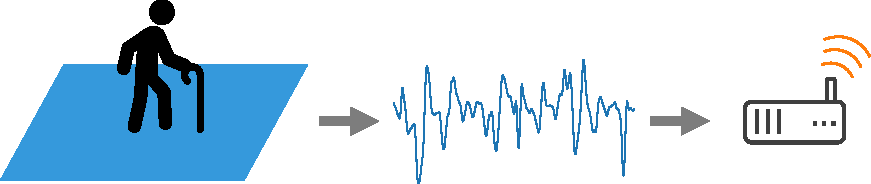
\includegraphics[width=0.95\linewidth]{schema_fall_detector.pdf}\\
        %         \onslide<1->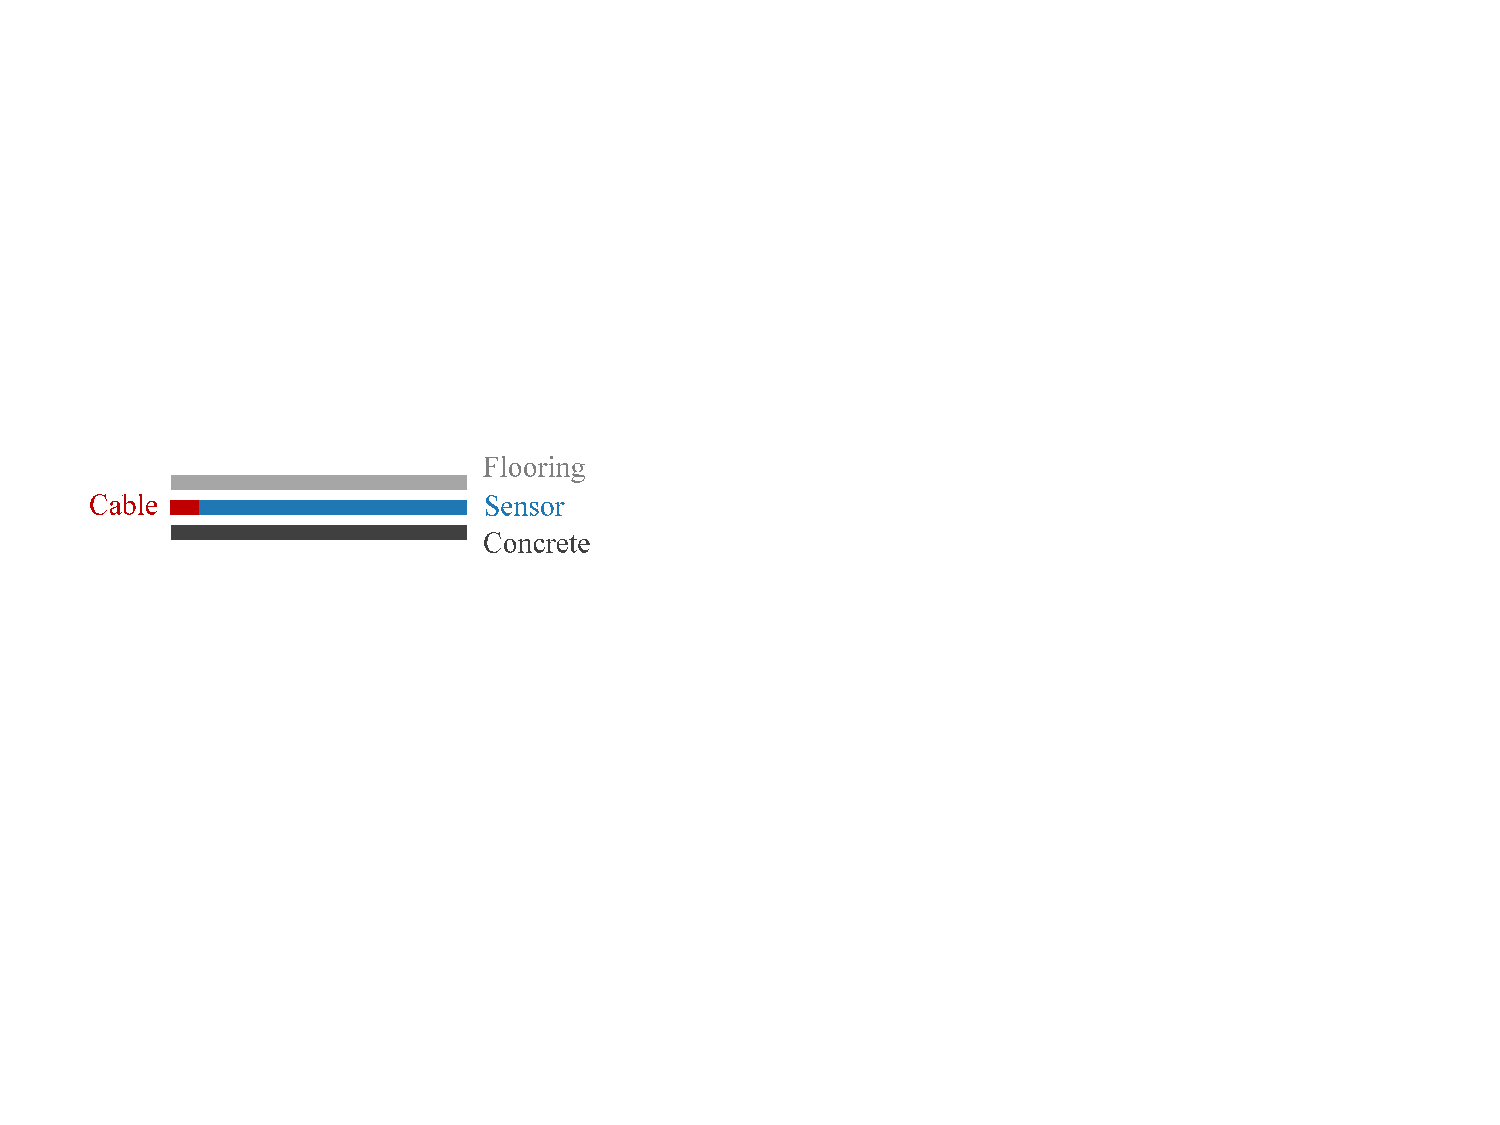
\includegraphics[width=0.4\linewidth, trim={20 230 430 200}, clip]{schema_sensor_installation_3.pdf}\\[5pt]
%                 \onslide<2->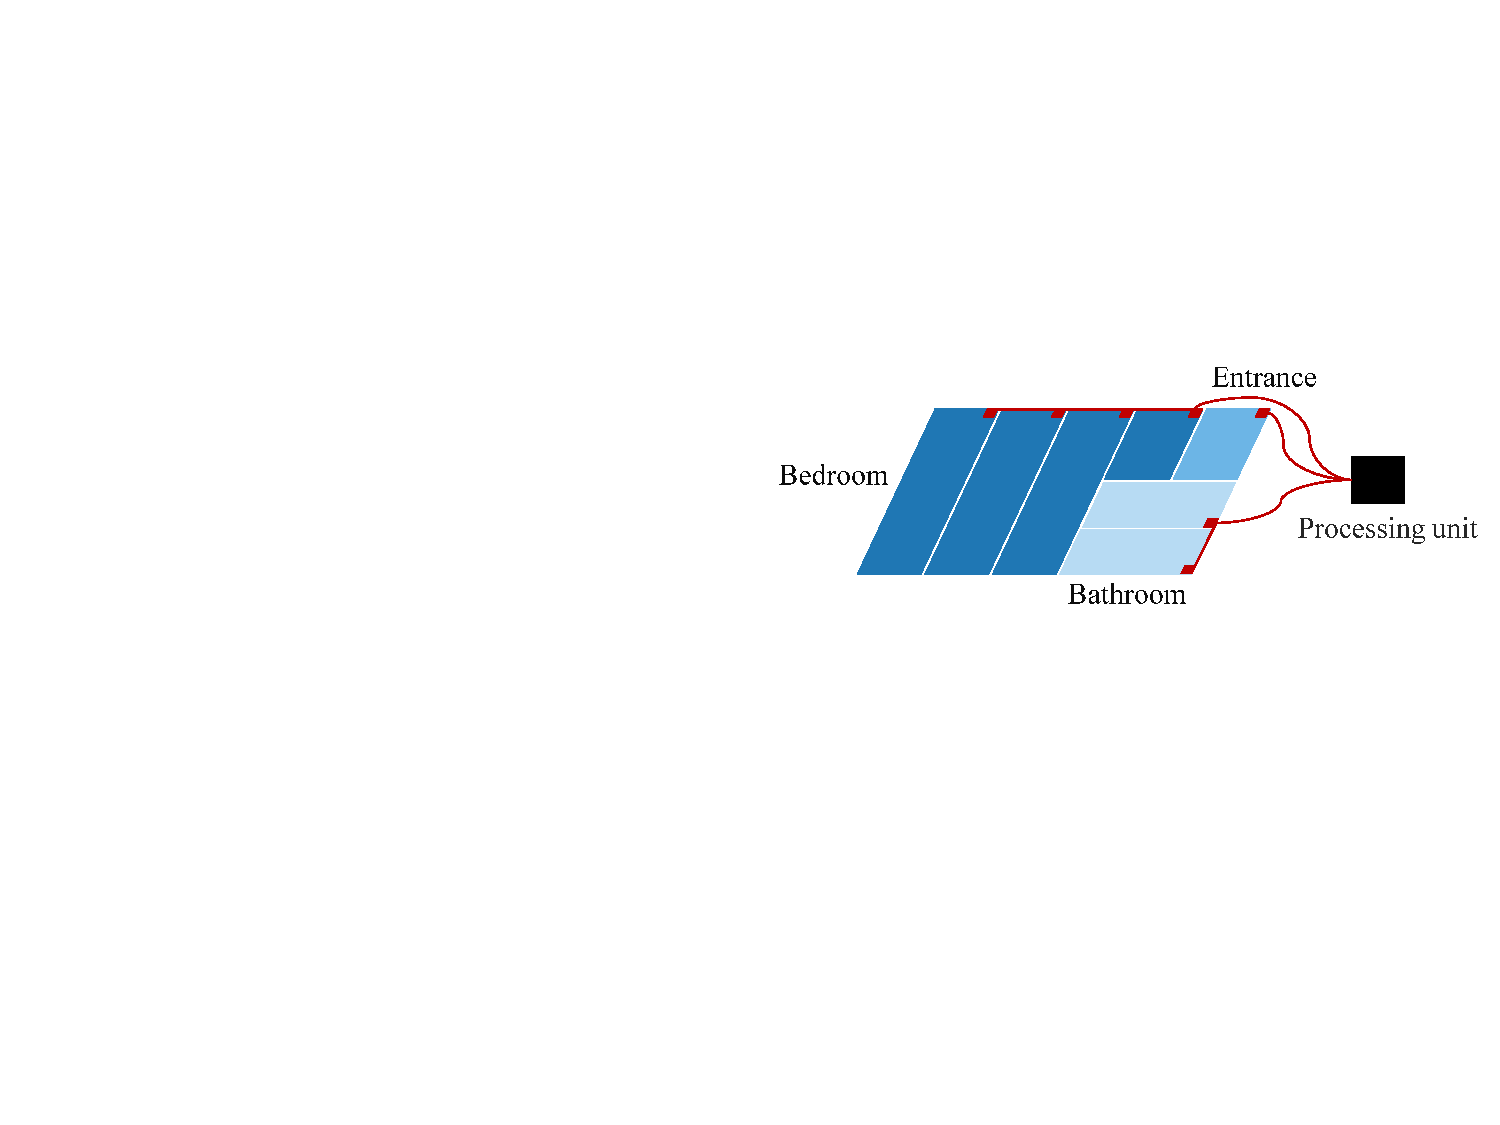
\includegraphics[width=0.4\linewidth, trim={360 230 5 160}, clip]{schema_sensor_installation_room_3.pdf}
        %         \onslide<2->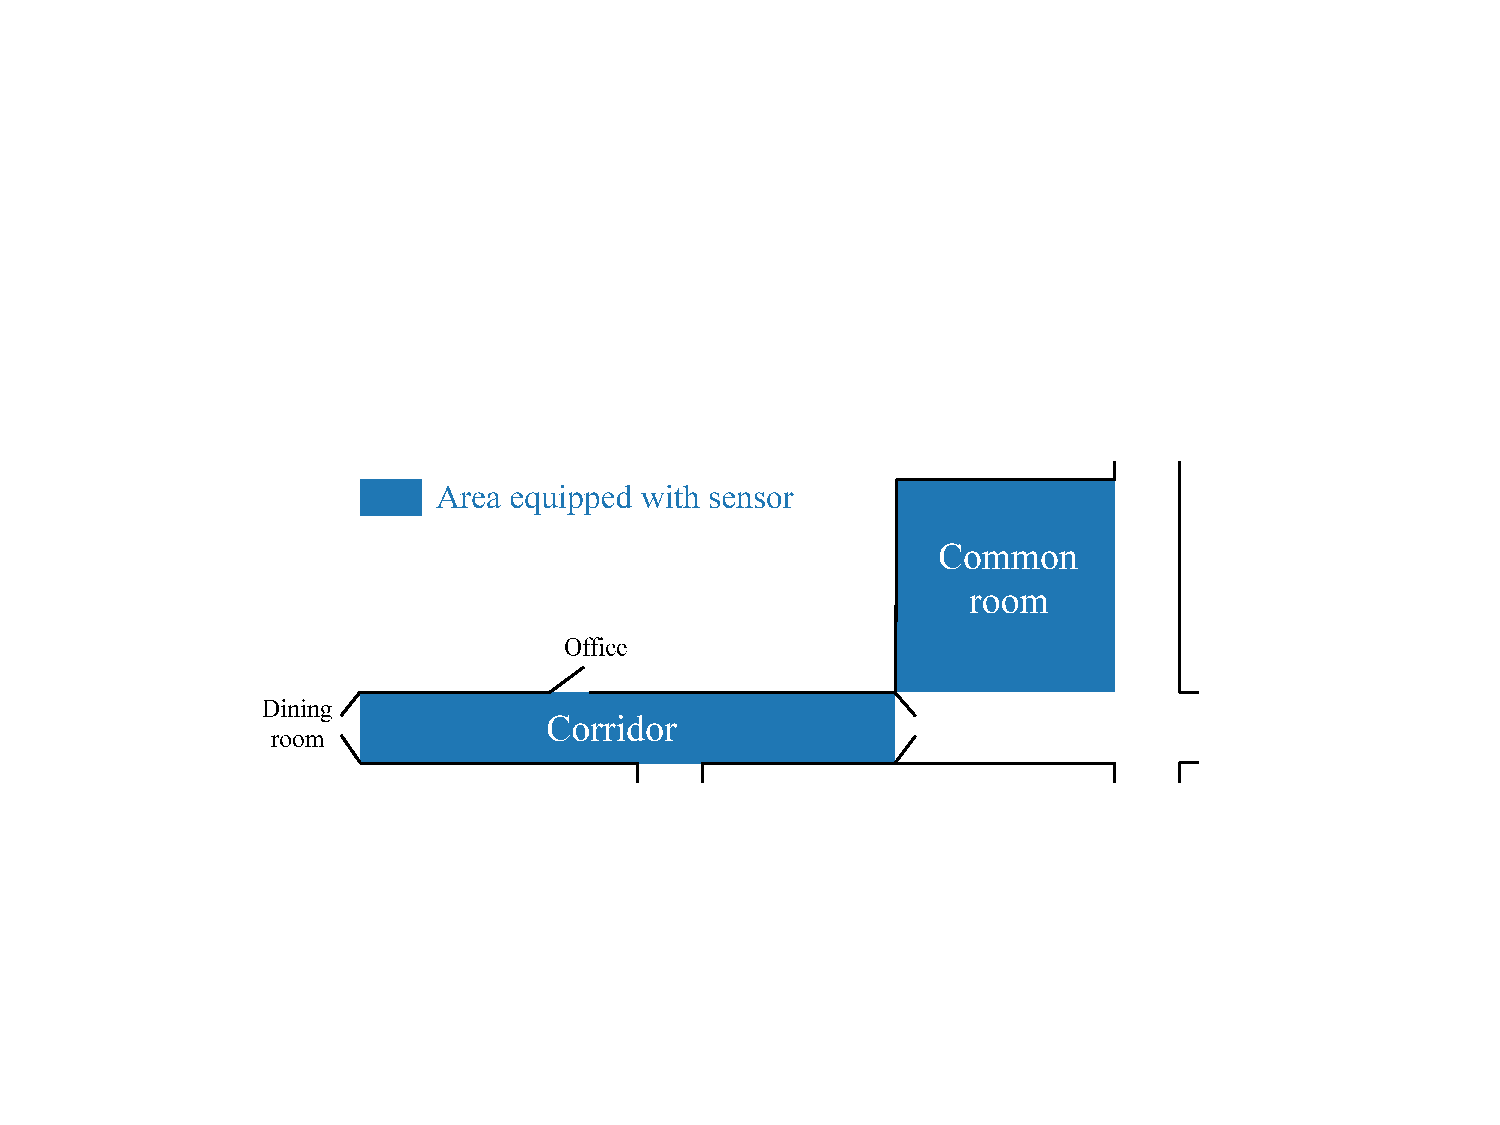
\includegraphics[width=0.6\linewidth, trim= 50 150 50 210, clip]{schema_couloir_plan_blue.pdf}
        %     \end{minipage}
        %     \caption{System installation in a nursing home.}
        %     \label{fig:schema_installation}
        \end{figure}
    \end{minipage}
\end{minipage}
\end{frame}

\begin{frame}{Introduction}{}
% \hspace{4cm}
\begin{minipage}[t]{\linewidth}
%     \centering
    \textbf{Motivation}
    \begin{itemize}
        \item Processing and understanding time series
        \begin{itemize}
            \item Proliferation of sensor-based systems
            \item Redundancy, interpretability, external pertubations
        \end{itemize}
        \item Real world application
        \begin{itemize}
            \item Real-time processing in a limited system
            \item Convenient hypotheses not granted
        \end{itemize}
    \end{itemize}
\end{minipage}

\renewcommand{\ratio}{0.4}
\begin{figure}[b]
    \centering
    \begin{minipage}{\linewidth}
        \centering
        \begin{minipage}{\ratio\linewidth}
            \centering
            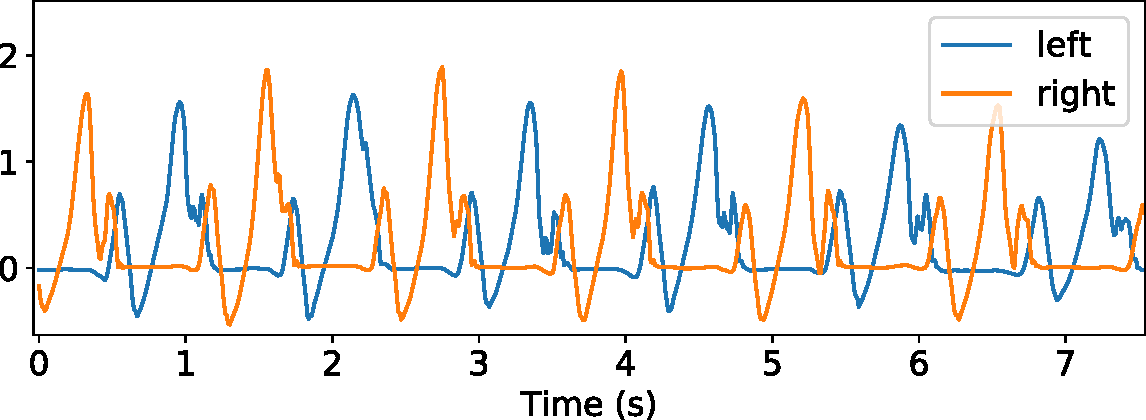
\includegraphics[width=0.91\linewidth]{signal_marche_accelerometre_left_right_epure.pdf}\\
            {\small (a)\; Foot-attached accelerometer}
        \end{minipage}
        \begin{minipage}{\ratio\linewidth}
            \centering
            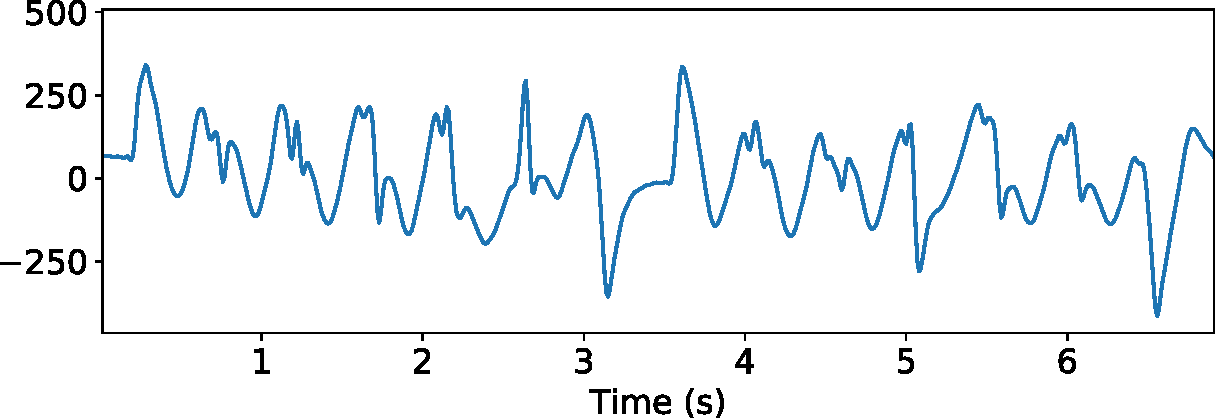
\includegraphics[width=\linewidth]{signal_marche_tarkett_epure.pdf}\\
            {\small (b)\; Tarkett's floor sensor}
        \end{minipage}
    \end{minipage}
%     \caption{Example of walk signals from different sensors.}
    \label{fig:introduction_signals_walk}
\end{figure}

\end{frame}

\section{A tour of monitoring systems}
\subsection{Systems}
\begin{frame}{A tour of monitoring systems}{Systems}
    



% \begin{minipage}[t]{\linewidth}
    \begin{minipage}[t]{0.49\linewidth}
        \vspace{0pt}
What makes a good monitoring system ?
        \begin{itemize}
            \item coverage and occlusion
            \item intrusiveness
            \item signal quality / information
            \item robustness
            \item ease of installation / use
            \item scalability
        \end{itemize}

    \end{minipage}\hfill
    \begin{minipage}[t]{0.49\linewidth}
        \vspace{0pt}
        \begin{overprint}
            \onslide<2>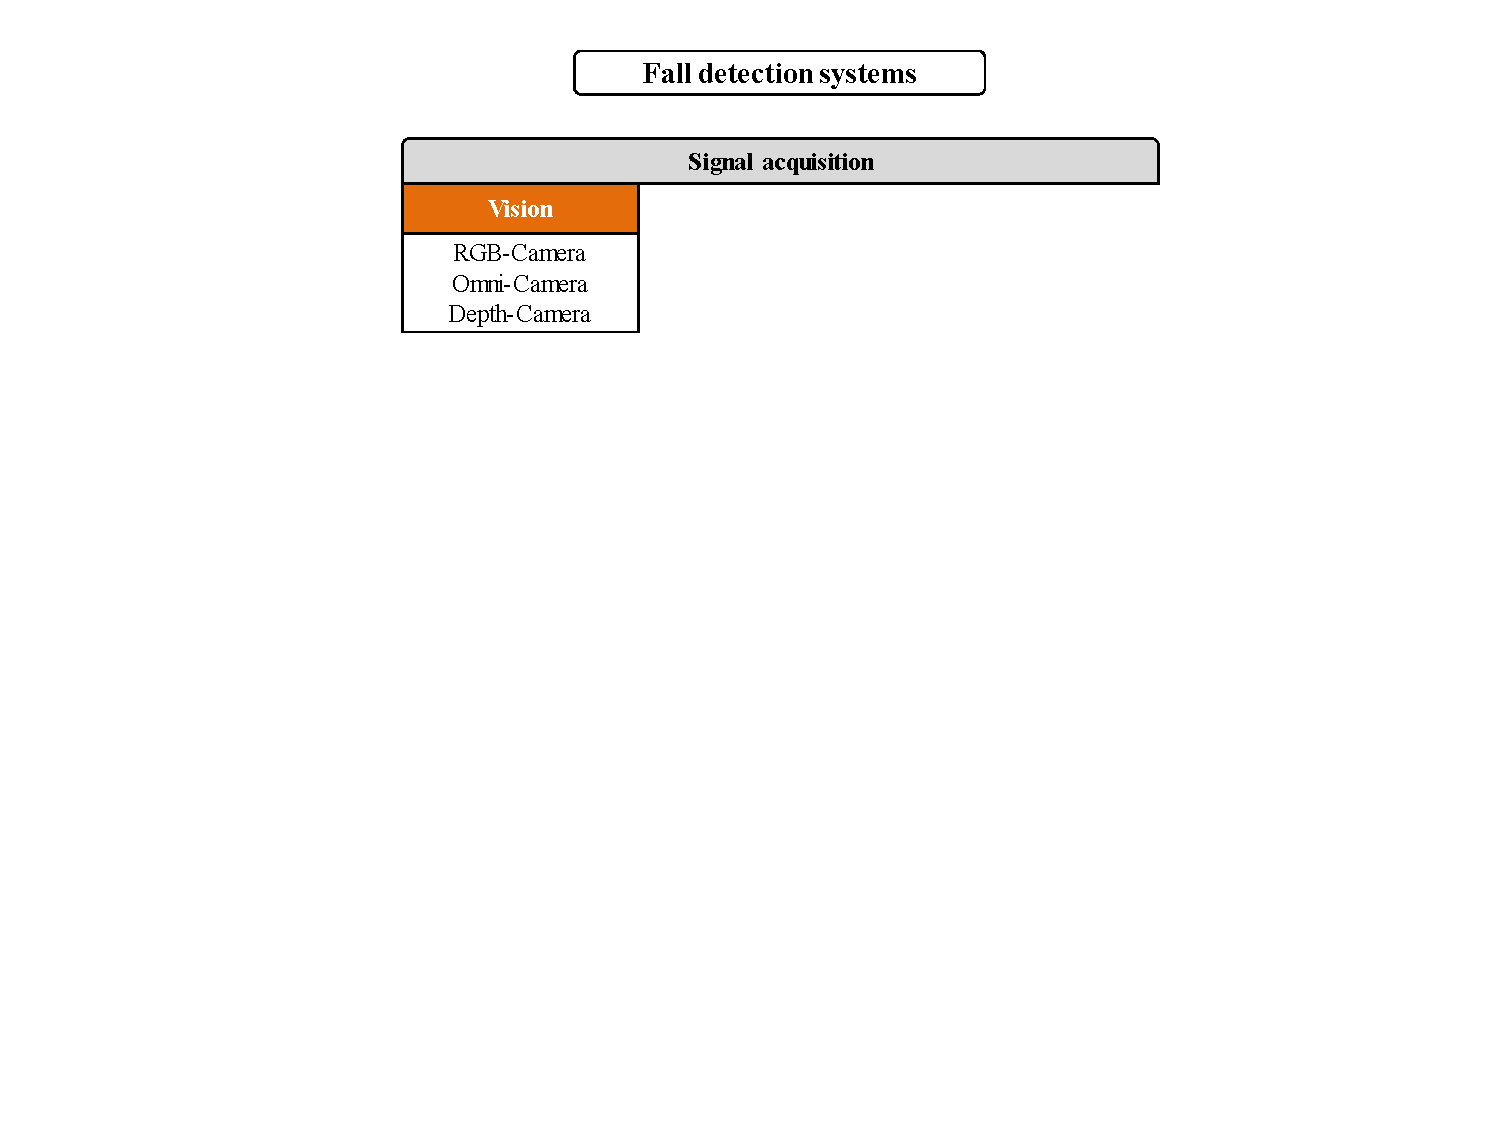
\includegraphics[width=\linewidth, trim={190 250 150 60}, clip]{fall_systems_1_1-14.pdf}
            \onslide<3>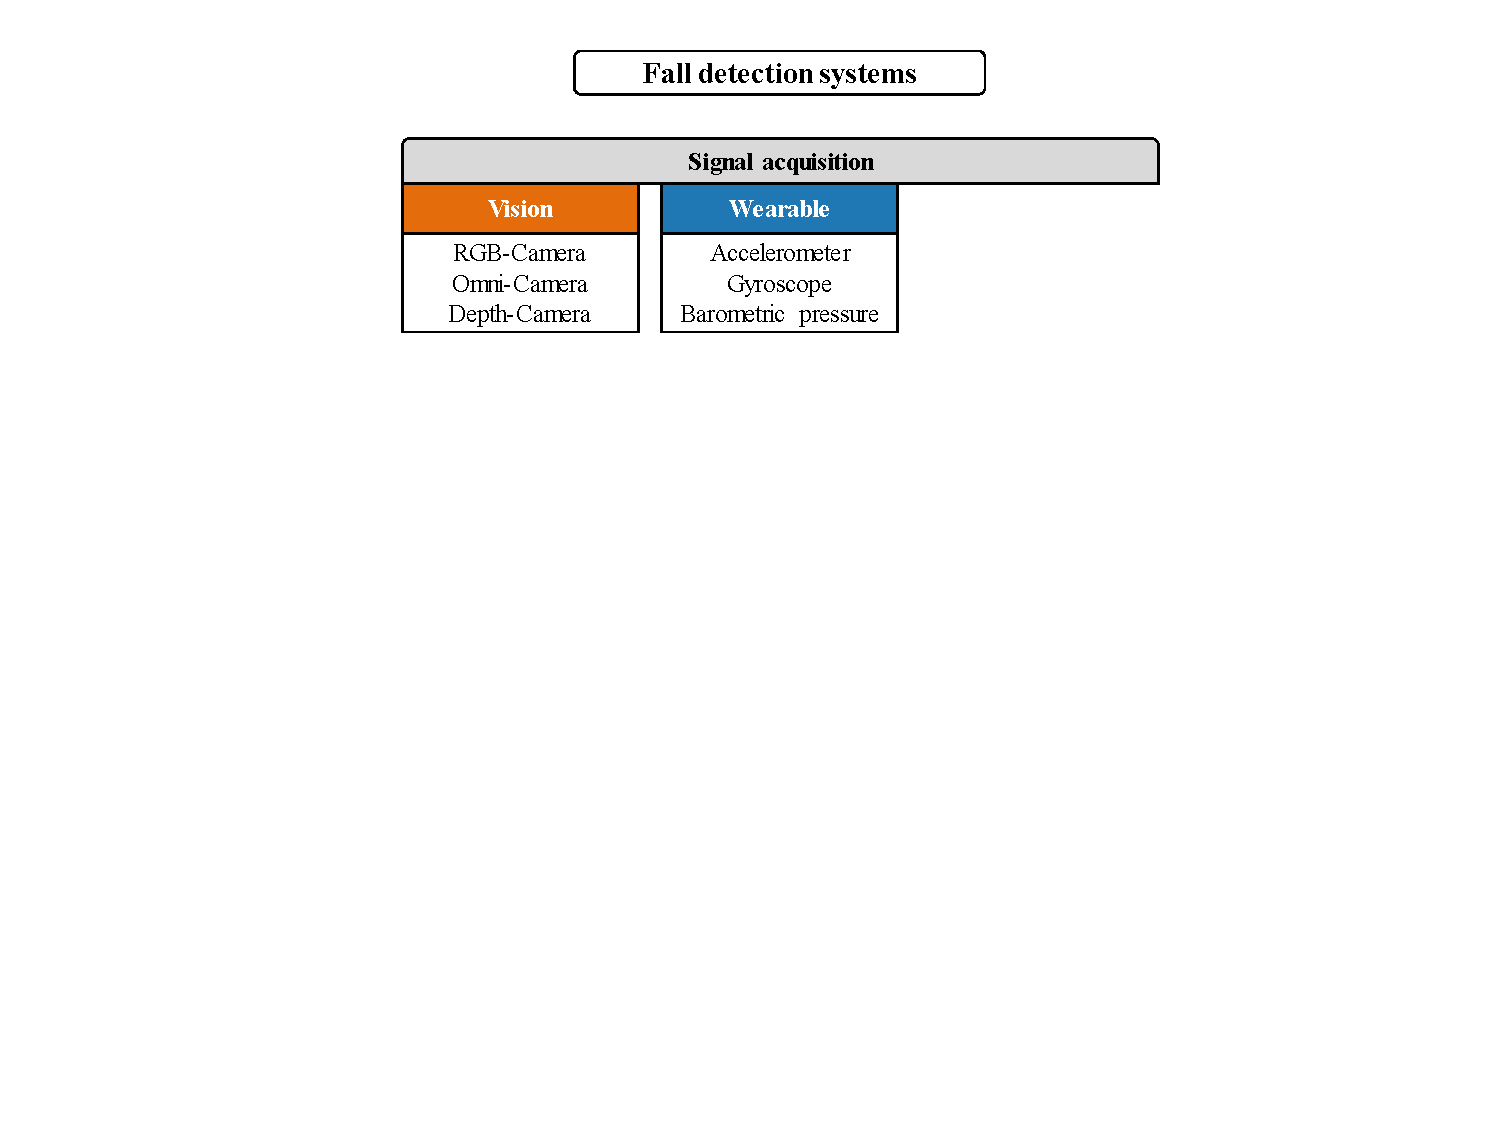
\includegraphics[width=\linewidth, trim={190 250 150 60}, clip]{fall_systems_1_2-14.pdf}
            \onslide<4>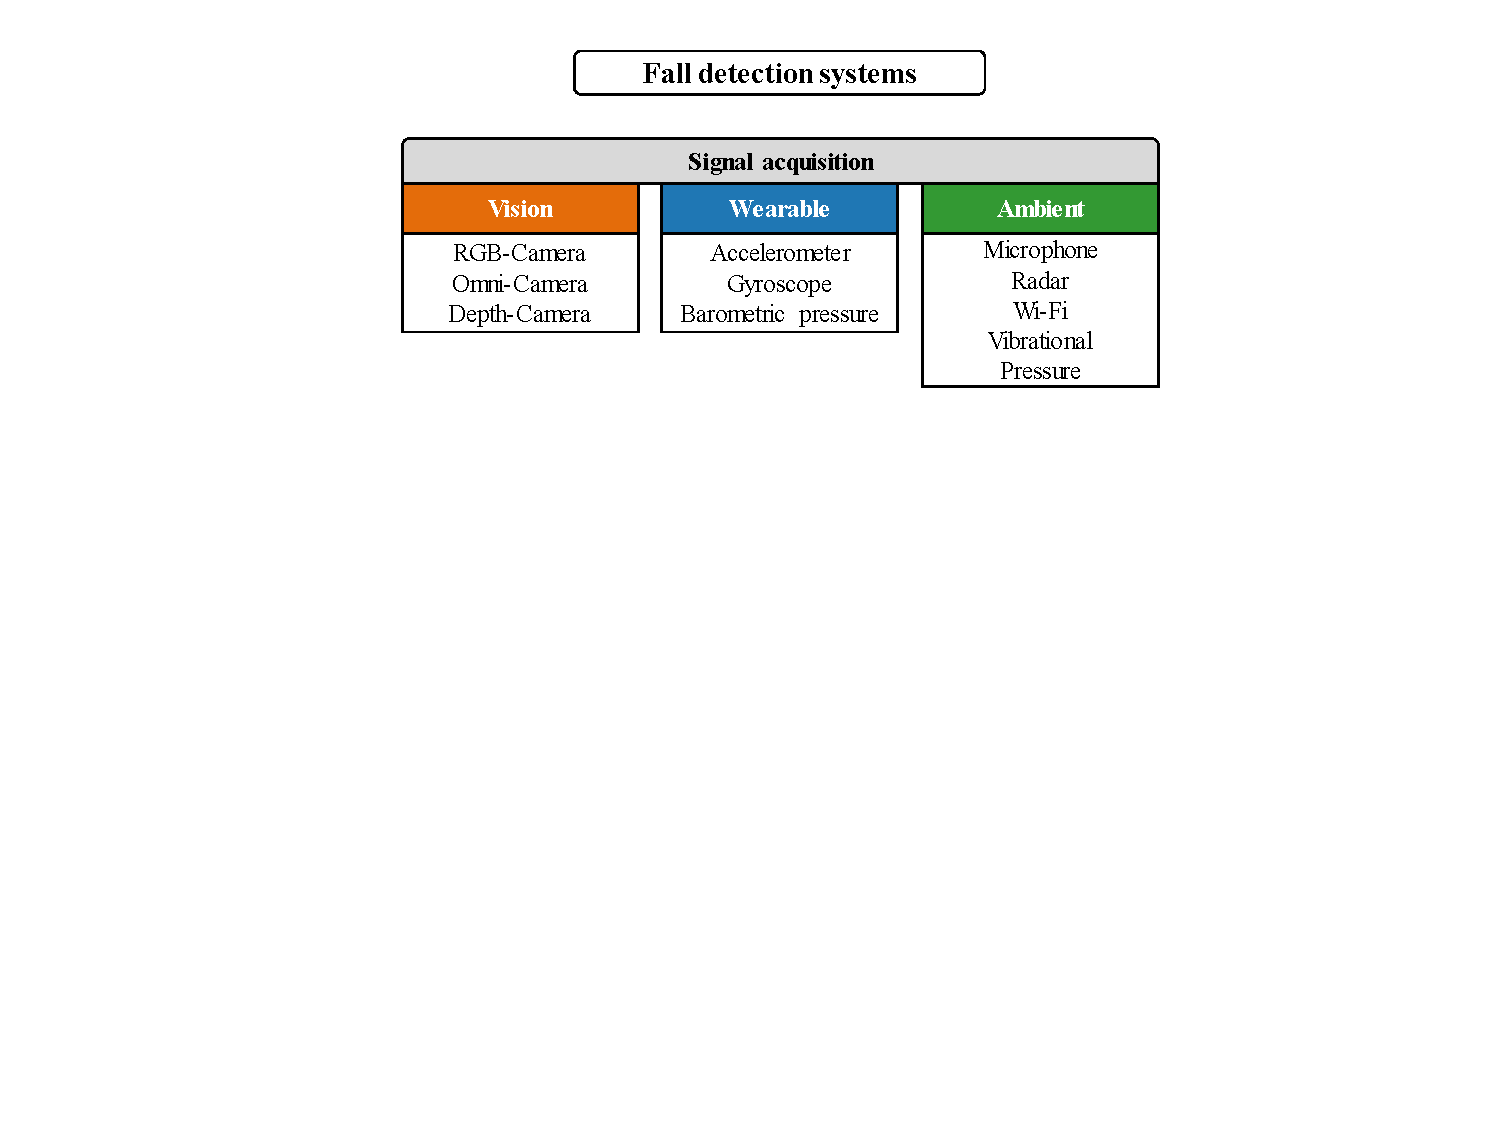
\includegraphics[width=\linewidth, trim={190 250 150 60}, clip]{fall_systems_1_3-14.pdf}
        \end{overprint}
    \end{minipage}
% \end{minipage}

\vspace{-0.8cm}
% \onslide<1>{
\renewcommand{\arraystretch}{1.1}
\newcommand{\myvar}{45}
\begin{table}[]
\centering
\footnotesize
% \small
    \begin{tabular}{l c c c c c c c}
%     \hline
    Criteria & \onslide<2->{\rotatebox{\myvar}{RGB cam} & \rotatebox{\myvar}{Depth cam}} & \onslide<3->{\rotatebox{\myvar}{Wearable}} & \onslide<4->{\rotatebox{\myvar}{Acoustic} & \rotatebox{\myvar}{Radar / Wi-Fi} & \rotatebox{\myvar}{Vibration} & \rotatebox{\myvar}{Floor}} \\
    \midrule
    Coverage/Occlusion & \onslide<2->{\starb\starw\starw & \starb\starw\starw} & \onslide<3->{\starb\starb\starb} & \onslide<4->{\starb\starb\starw & \starb\starw\starw & \starb\starb\starb & \starb\starb\starb} \\
    Intrusiveness & \onslide<2->{\starb\starw\starw & \starb\starw\starw} & \onslide<3->{\starb\starb\starw} & \onslide<4->{\starb\starw\starw & \starb\starb\starw & \starb\starb\starb & \starb\starb\starb} \\
    Signal quality / info &\onslide<2->{\starb\starb\starb & \starb\starb\starb} & \onslide<3->{\starb\starb\starw} & \onslide<4->{\starb\starb\starw & \starb\starw\starw & \starb\starb\starw & \starb\starb\starw} \\
    Robustness & \onslide<2->{\starb\starb\starw & \starb\starb\starb} & \onslide<3->{\starb\starb\starb} & \onslide<4->{\starb\starw\starw & \starb\starw\starw & \starb\starw\starw & \starb\starb\starw} \\
    Ease of instal. / use & \onslide<2->{\starb\starw\starw & \starb\starw\starw} & \onslide<3->{\starb\starb\starw} & \onslide<4->{\starb\starb\starw & \starb\starb\starw & \starb\starb\starb & \starb\starw\starw} \\
    Scalability & \onslide<2->{\starb\starw\starw & \starb\starw\starw} & \onslide<3->{\starb\starb\starb} & \onslide<4->{\starb\starb\starw & \starb\starw\starw & \starb\starb\starw & \starb\starb\starb} \\
    \midrule
    \end{tabular}
% \caption{Sensors evaluation over key criteria for patient monitoring systems.}
\label{tab:fall_detection_sensors_comparison}
\end{table}
\renewcommand{\arraystretch}{1.0}
% }

\end{frame}

\subsection{Processing}
\begin{frame}{A tour of monitoring systems}{Processing}

% \begin{minipage}[t]{\linewidth}
    \begin{minipage}[t]{0.49\linewidth}
    \vspace{0pt}
    How to process the inputs ?
    \begin{itemize}
        \item All systems use feature extraction
        \item The ``level'' of feature engineering depends on the complexity / dimensionality of the input signal
    \end{itemize}
    How to deal with processed signals ?
    \begin{tcolorbox}[height=4.2cm]
        \textbf{Time series classification}\\[-5pt]
        \begin{enumerate}
            \item Series as \emph{sequences}
            \begin{itemize}
                \item Distance-based methods
            \end{itemize}
            \item Series as \emph{feature vectors}
            \begin{itemize}
                \item Computing several measures over a fixed size
                \item Classification models
                (Anomaly detection, classical supervised models...)
            \end{itemize}
        \end{enumerate}
    \end{tcolorbox}
%     \vfill
%     \vspace{10cm}
    \end{minipage}
    \hfill
    \begin{minipage}[t]{0.49\linewidth}
    \vspace{0pt}
        \begin{overprint}
%             \onslide<3>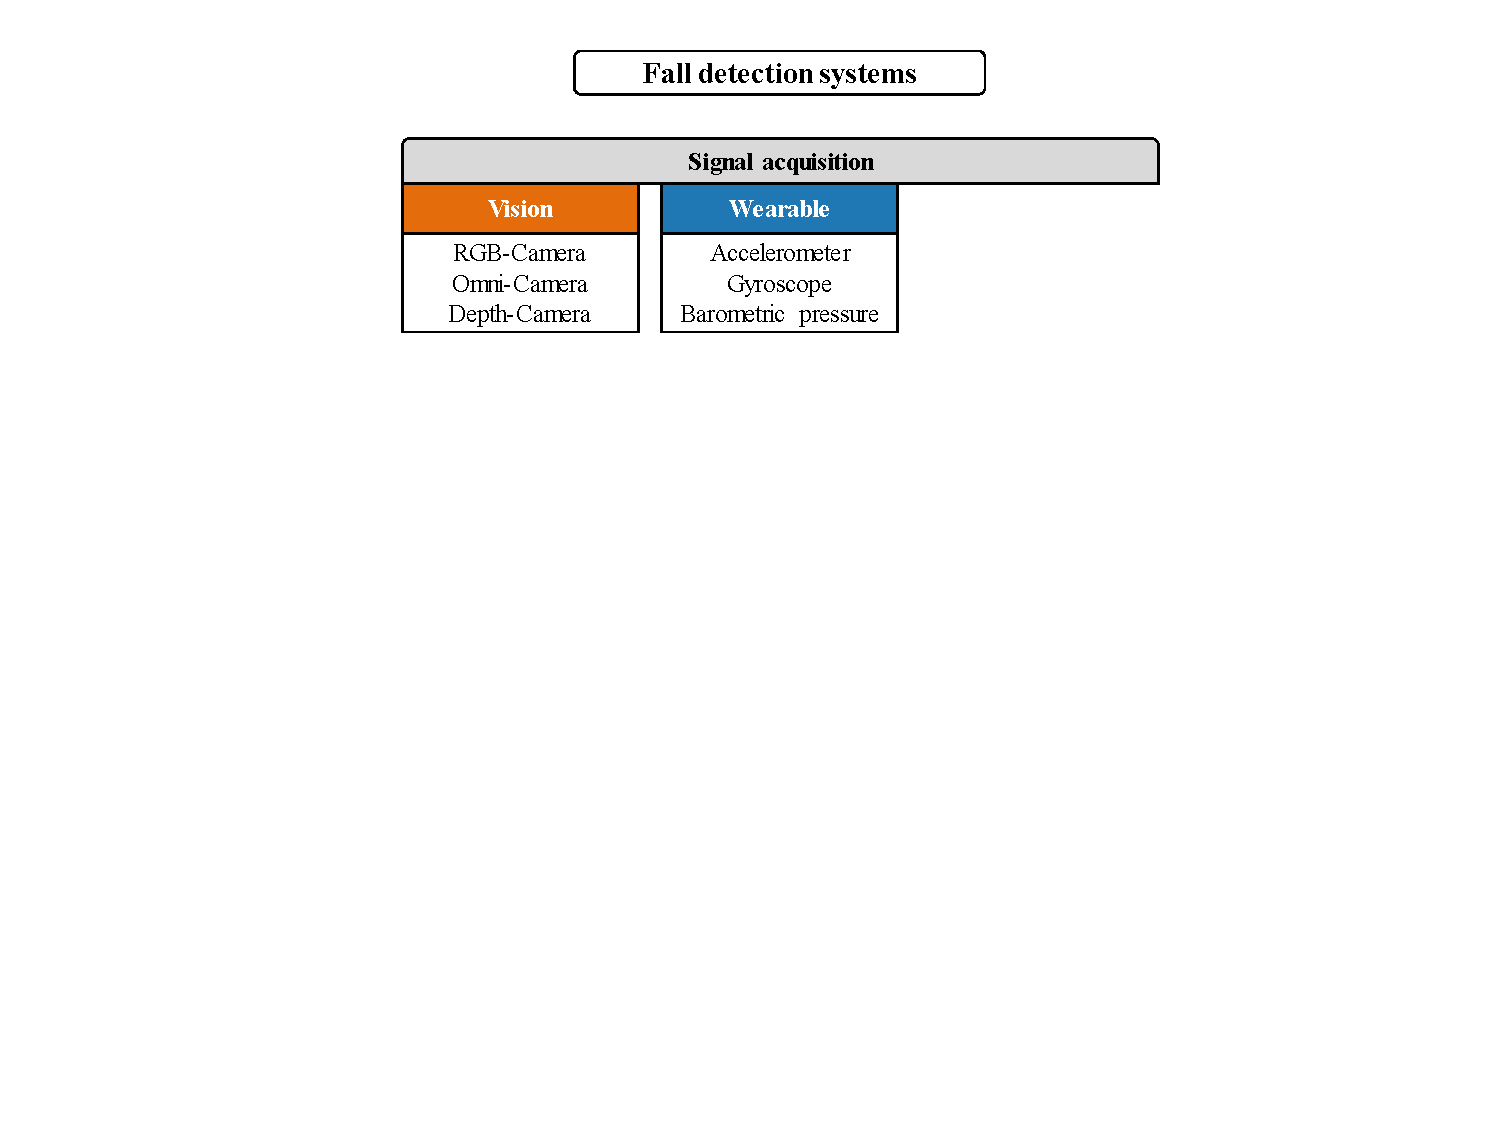
\includegraphics[width=\linewidth, trim={190 50 150 20}, clip]{fall_systems_1_2-14.pdf}
%             \onslide<4>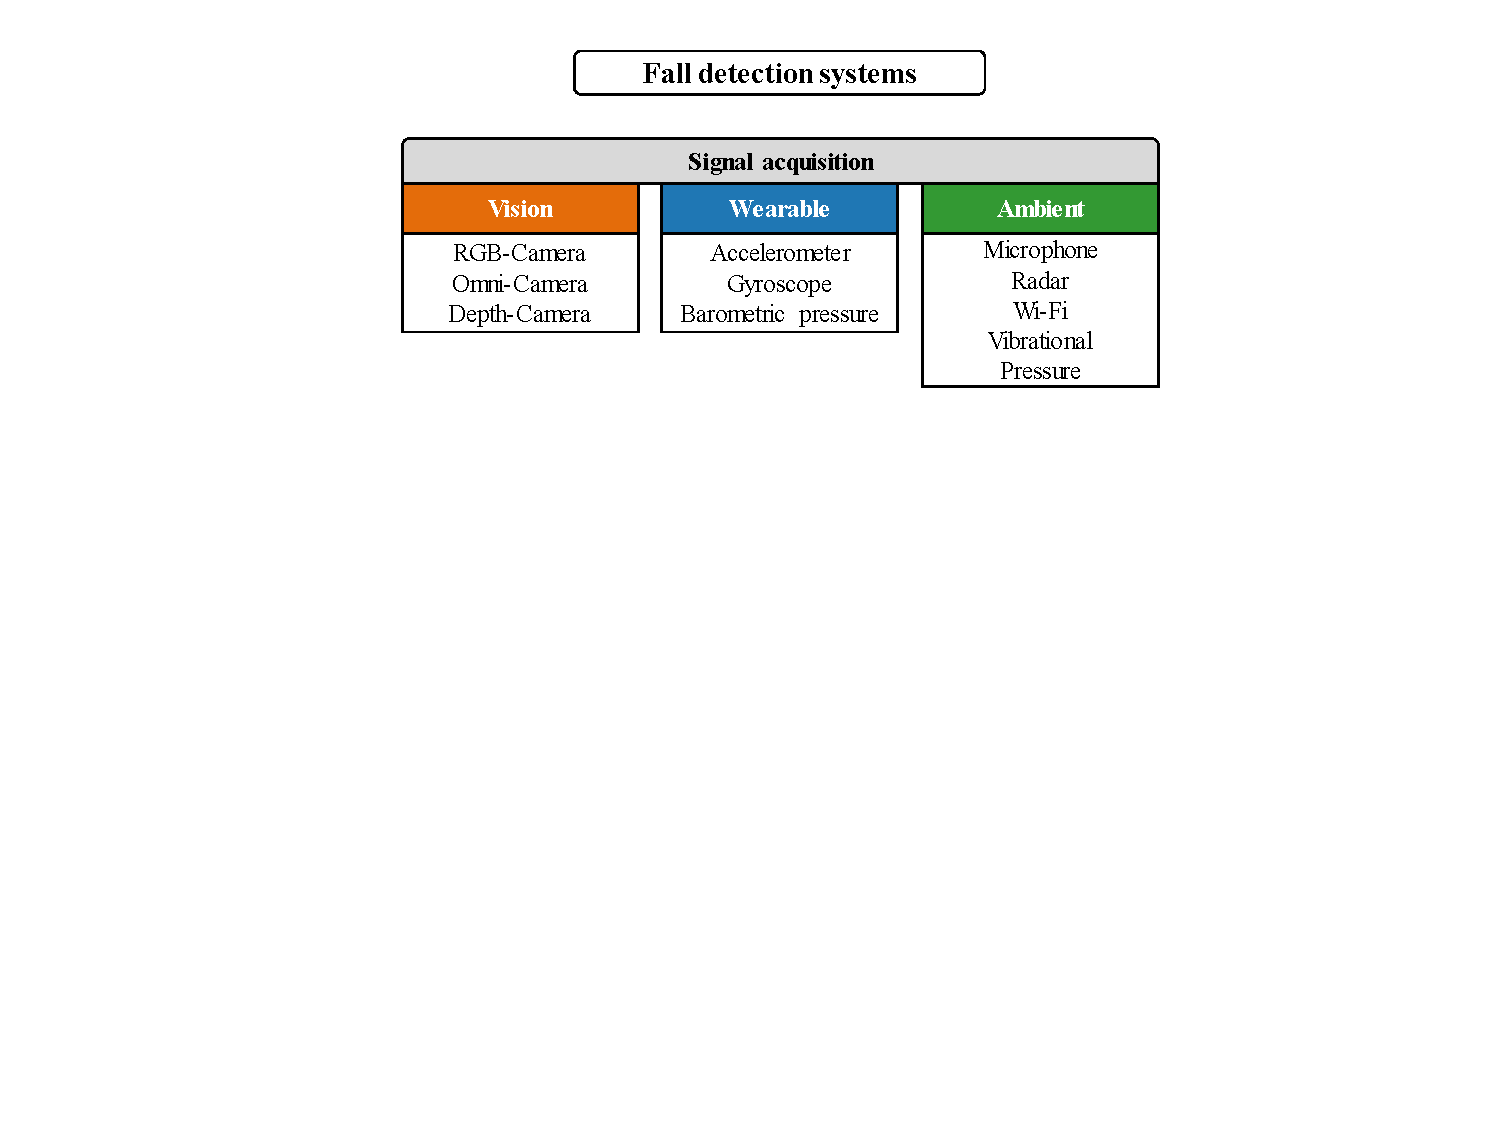
\includegraphics[width=\linewidth, trim={190 50 150 20}, clip]{fall_systems_1_3-14.pdf}
            \onslide<1>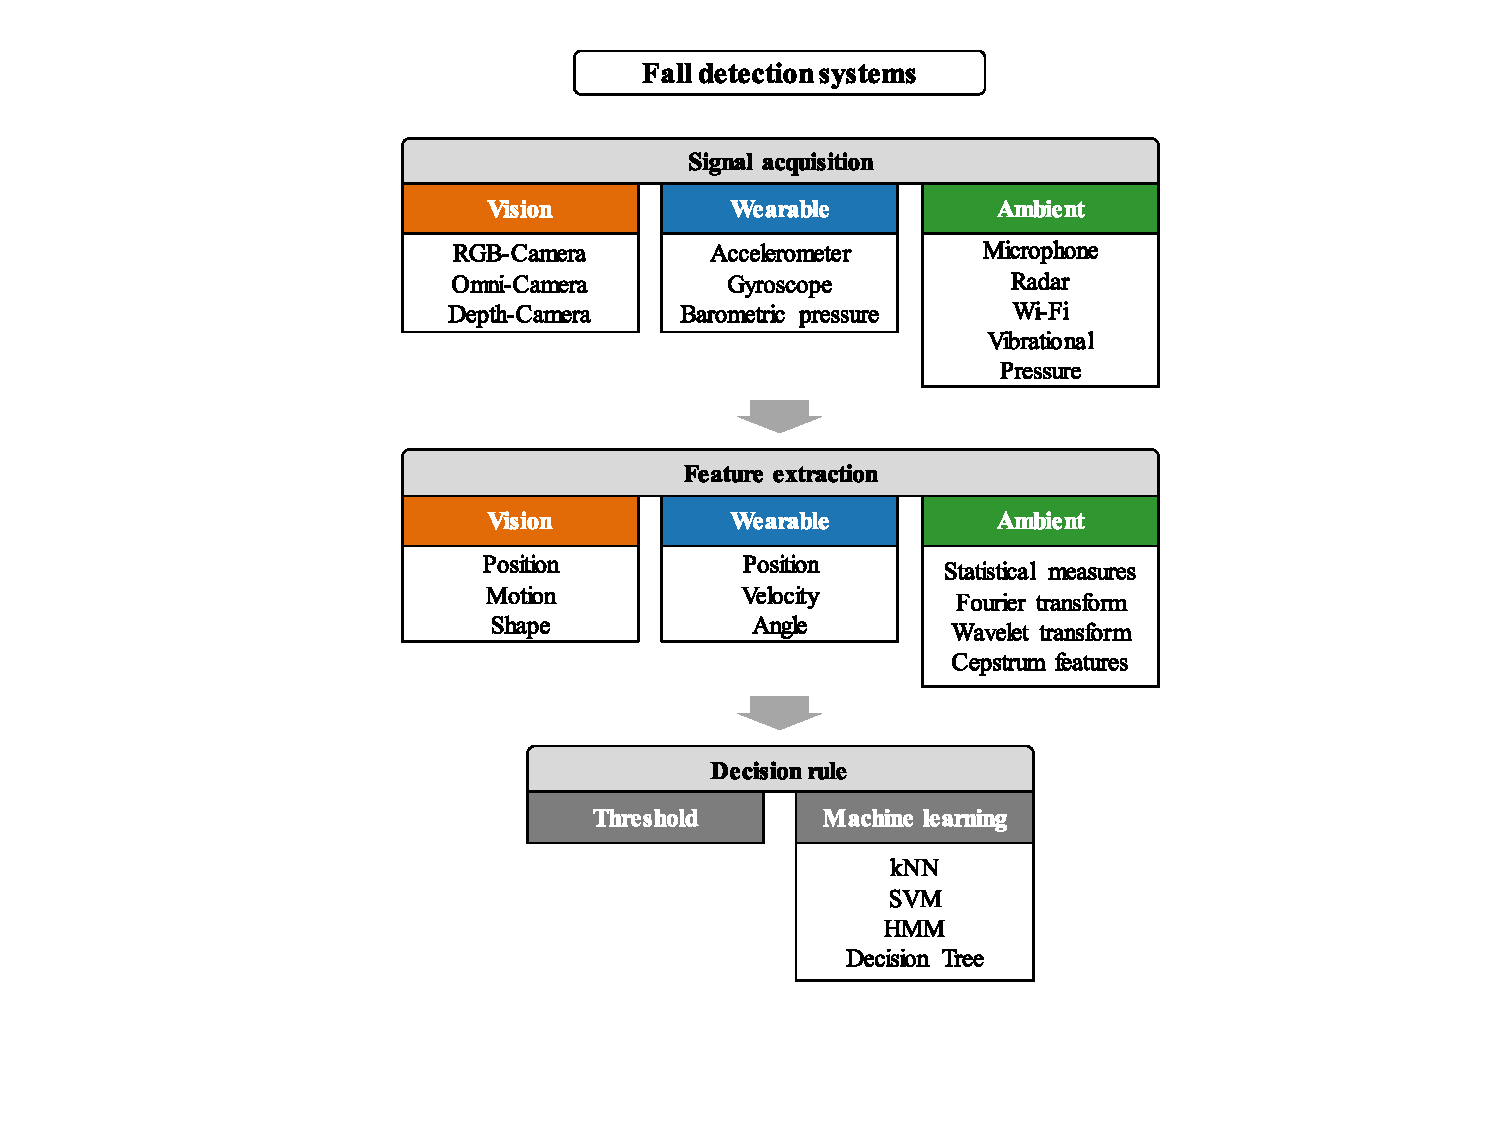
\includegraphics[width=\linewidth, trim={190 50 150 60}, clip]{fall_systems_3-14.pdf}
        \end{overprint}
    \end{minipage}
% \end{minipage}
\end{frame}

\begin{frame}{A tour of monitoring systems}{Tarkett sensor}
\end{frame}










\begin{frame}{Introduction}{}
\begin{itemize}
    \item \textbf{Issue}: one-dimensional signals for large areas
    \item Goal: Classify elderly from other individuals
%     using a convolutional neural network 
    \begin{itemize}
        \item Most signals are made of walks of staff individuals
    \end{itemize}
    \item \textbf{Subtask}: Bring the model's attention over step-related signals
\end{itemize}
\begin{itemize}
    \item A model to recognize steps ?
\end{itemize}

\pause
\begin{figure}[h]
    \begin{minipage}{\linewidth}
        \centering
        \begin{minipage}{0.49\linewidth}
            \centering
            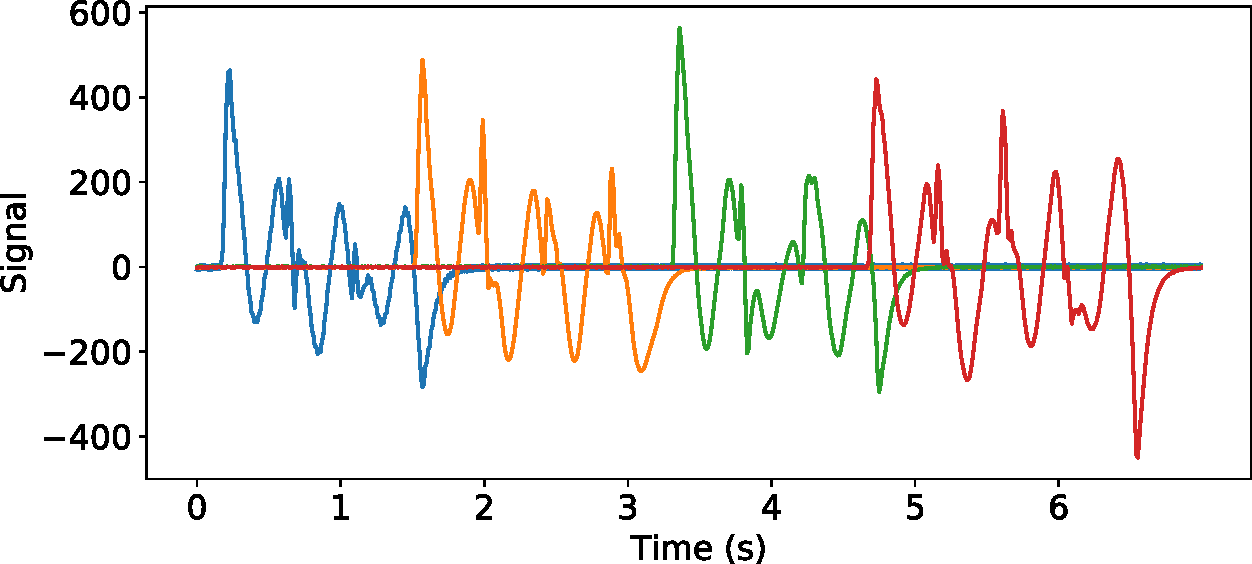
\includegraphics[width=0.9\linewidth]{signal_walk_young_female_before_preproc_2.pdf}\\
            {\small (a)\; Raw signal}
        \end{minipage}
        \begin{minipage}{0.49\linewidth}
            \centering
            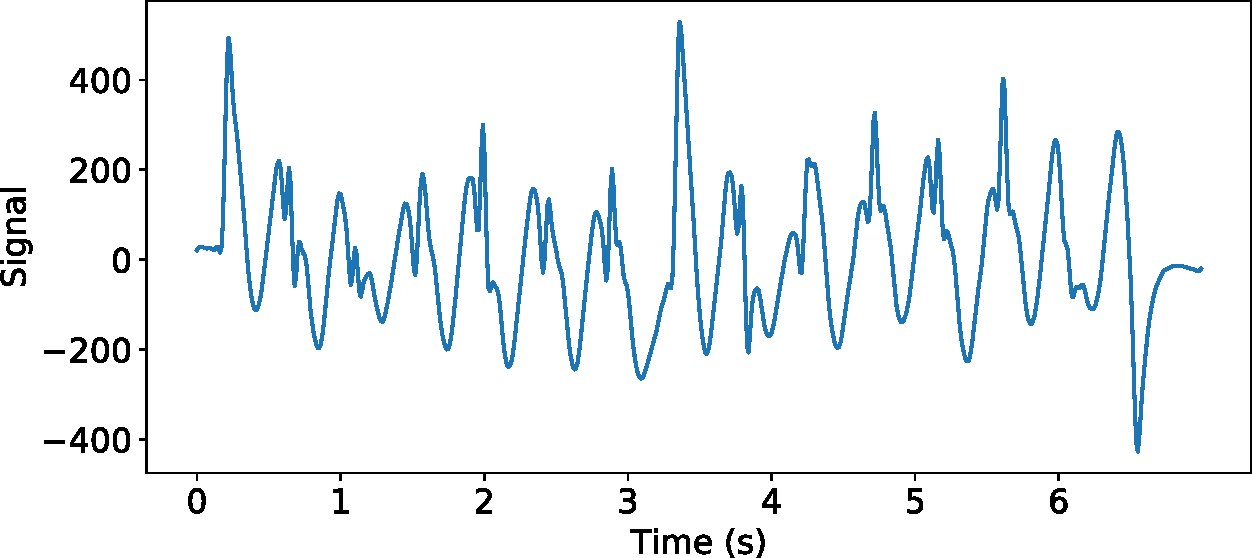
\includegraphics[width=0.9\linewidth]{signal_walk_young_female_after_preproc_2.pdf}\\
            {\small (b)\; Preprocessed signal}
        \end{minipage}
    \end{minipage}
    \caption{Healthy individual walking on the sensor.}
    \label{fig:walk_class_ex_preprocessing}
\end{figure}
\begin{itemize}
    \item Signals are complex
    \item How to \textbf{localize} steps ?
    \item \textbf{This presentation:} A step detector using convolutional neural network: Step Proposal Network
\end{itemize}

\end{frame}
%
% ---------------------------------------------------------------
\section{Step proposal network}

% \subsection{Architecture}

\subsection{Region proposal network}

\begin{frame}[noframenumbering]{\ }
\hfill
\parbox[t]{.85\textwidth}{
%   \large
  \begin{minipage}[c][0.65\textheight]{\textwidth}
  \tableofcontents[currentsection, subsectionstyle=show/shaded/shaded]
  \end{minipage}
}
\end{frame}


\begin{frame}{Region proposal network}{Object detection}
\begin{itemize}
    \item Classification: What is the image class ?
    \pause
    \item Object detection: Where are the objects and what are they classes ?
    \pause
    \item How to efficiently localize objects ?
    \item Proposal models \cite{hosang2016what}
    \item Faster R-CNN \cite{ren2015faster}
\end{itemize}
\begin{figure}
    \onslide<1->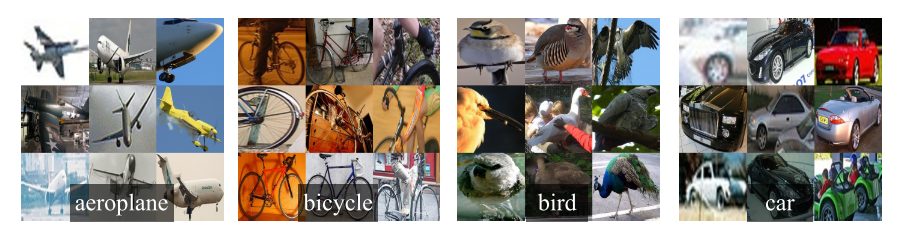
\includegraphics[width=\ratio\linewidth, trim=0 0 340 0, clip]{rcnn_images.png}
    \onslide<2->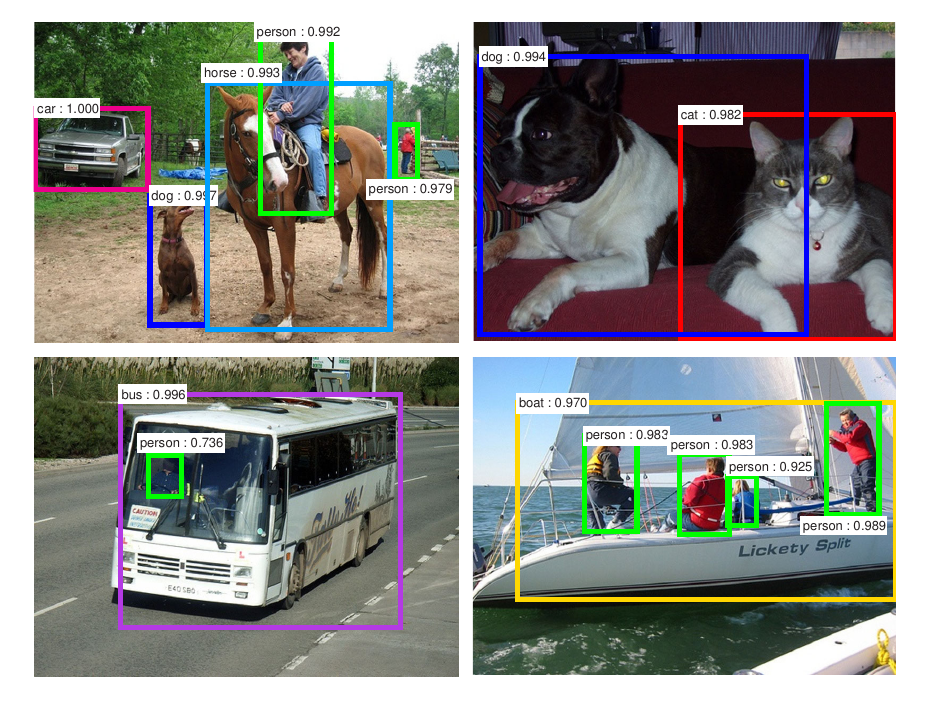
\includegraphics[width=\ratio\linewidth]{faster_rnn_rpn_imageoutputs.png}
    \onslide<1->\caption{Classification vs Object detection. Source: \cite{girshick2014rich},  \cite{ren2015faster}}
\end{figure}

\end{frame}

\begin{frame}{Region proposal network}{Faster R-CNN}
\begin{itemize}
    \item Main idea: proposals are generated by a CNN called Region Proposal Network
    \pause
    \item A sliding window is passed: multiple \emph{anchors} over each location (various sizes and scales)
    \item Two layers: Classification (Object / Not Object) and Regression (anchor coordinates)
\end{itemize}
    
\renewcommand{\ratio}{0.45}
\centering
\begin{figure}
    \onslide<1->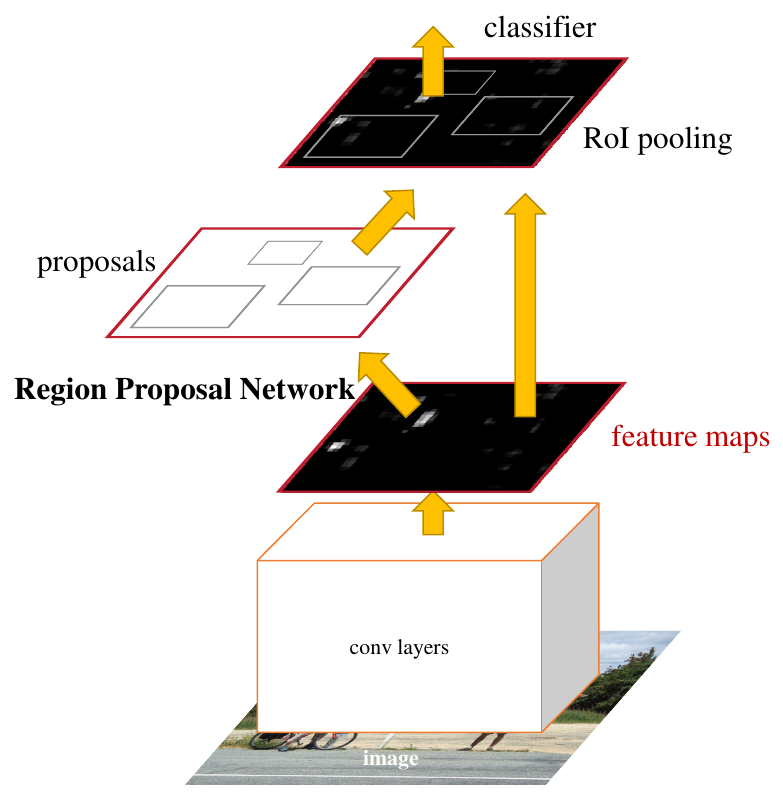
\includegraphics[width=0.4\linewidth]{faster_rnn_wholenetwork.png}
    \onslide<2->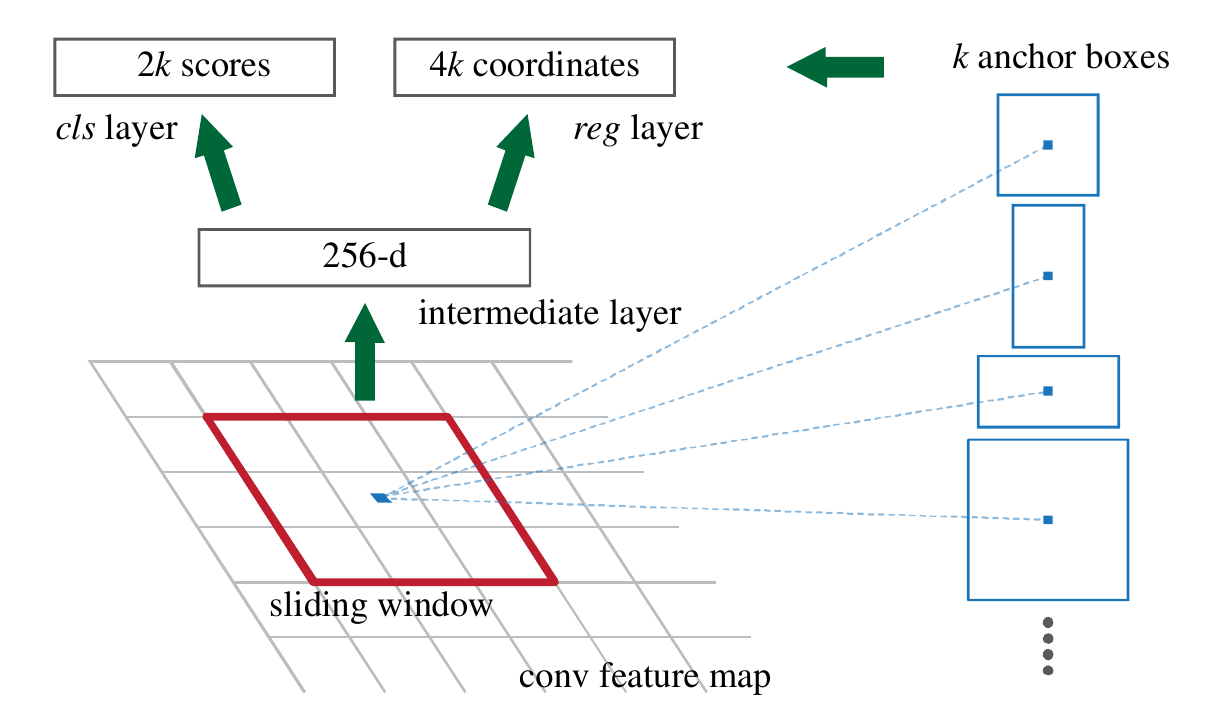
\includegraphics[width=0.55\linewidth]{faster_rnn_rpn.png}
    \onslide<1->\caption{Region proposal network. Source: \cite{ren2015faster}}
\end{figure}

\end{frame}

\subsection{Main architecture}

\begin{frame}[noframenumbering]{\ }
\hfill
\parbox[t]{.85\textwidth}{
%   \large
  \begin{minipage}[c][0.65\textheight]{\textwidth}
  \tableofcontents[currentsection, subsectionstyle=show/shaded/shaded]
  \end{minipage}
}
\end{frame}

\begin{frame}{Step proposal network}{Main architecture}

\begin{itemize}
    \item Directly inspired from RPN
    \item Simple architecture with three hidden layers, all \textbf{convolutional}
    \item Output: probability of having a step at a specific window location and size
    \begin{itemize}
    \item Here 3 sizes and all discrete locations are considered
    \end{itemize}
\end{itemize}

\begin{figure}[h]
    \begin{minipage}{\linewidth}
        \centering
        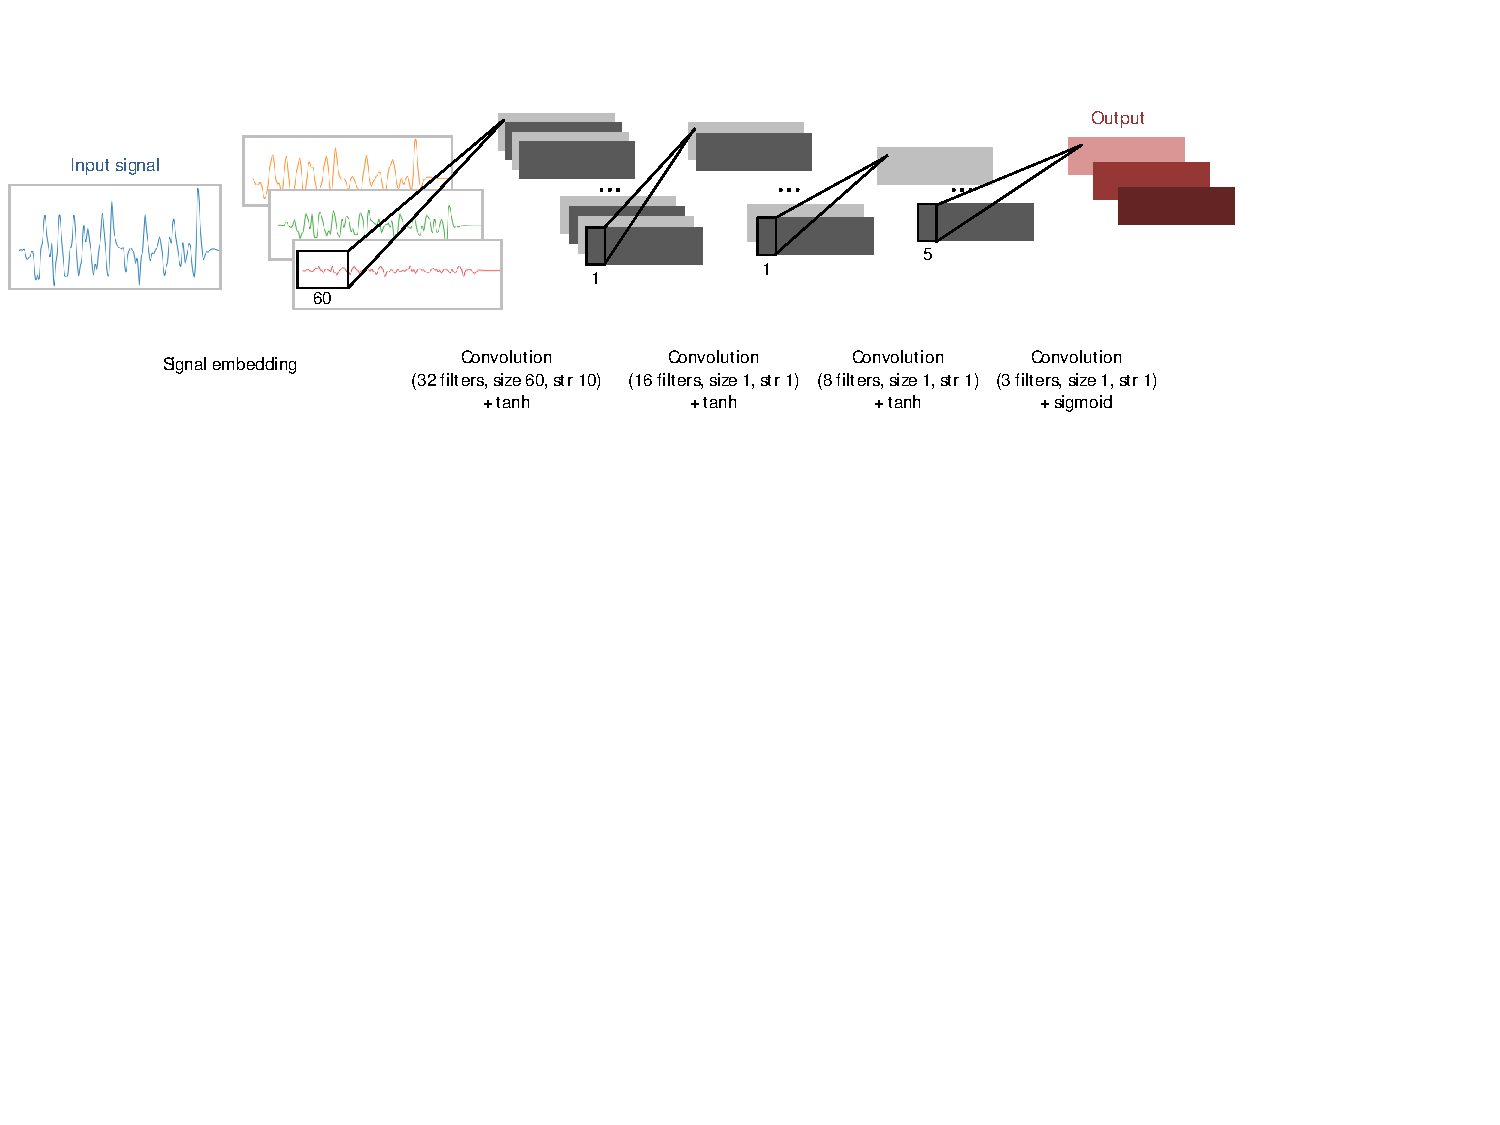
\includegraphics[width=\linewidth, trim= 0 340 120 40, clip]{schema_cnn_rpn}
        \caption{Architecture of \subalgo.}
        \label{fig:walk_class_cnn_spn}
    \end{minipage}
\end{figure}

\pause
\begin{itemize}
    \item Use the convolutional representation to ``boost'' training
    \item First layer (Signal embedding) of \subalgo is trained \textbf{separately} using convolutional dictionary learning
\end{itemize}
    
\end{frame}

\subsection{Signal embedding}

\begin{frame}[noframenumbering]{\ }
\hfill
\parbox[t]{.85\textwidth}{
%   \large
  \begin{minipage}[c][0.65\textheight]{\textwidth}
  \tableofcontents[currentsection, subsectionstyle=show/shaded/shaded]
  \end{minipage}
}
\end{frame}


\begin{frame}{Signal embedding}{Convolutional dictionary learning}
\begin{minipage}[t]{0.45\linewidth}
    \begin{itemize}
        \item $\bfs$ : data to be represented
        \item Objective : find $M$ atoms $\bfd_m$ and activation signals $\bfx_m$ such that
        $$\bfs \approx \sum_{m=1}^{M}\bfx_m * \bfd_m$$
        \item $*$ : convolution
    \end{itemize}
    \pause[3]
    CDL general problem:
    \begin{gather*}\label{eq:cdl_baseform}
    \argmin_{\bfx_m,\bfd_m} \frac{1}{2} \left\| \sum_{m=1}^{M} \bfx_{m} * \bfd_m - \bfs \right\|_2^2 + \lambda \sum_{m=1}^{M} \|\bfx_m \|_1 \ \\
        \text{s.t.}\quad \| \bfd_m\|_2 \leq 1 \quad \forall m \;. \nonumber
    \end{gather*}
\end{minipage}\hfill
\begin{minipage}[t]{0.4\linewidth}
    \centering
    \pause[2]
    \begin{figure}[h]
        \centering
        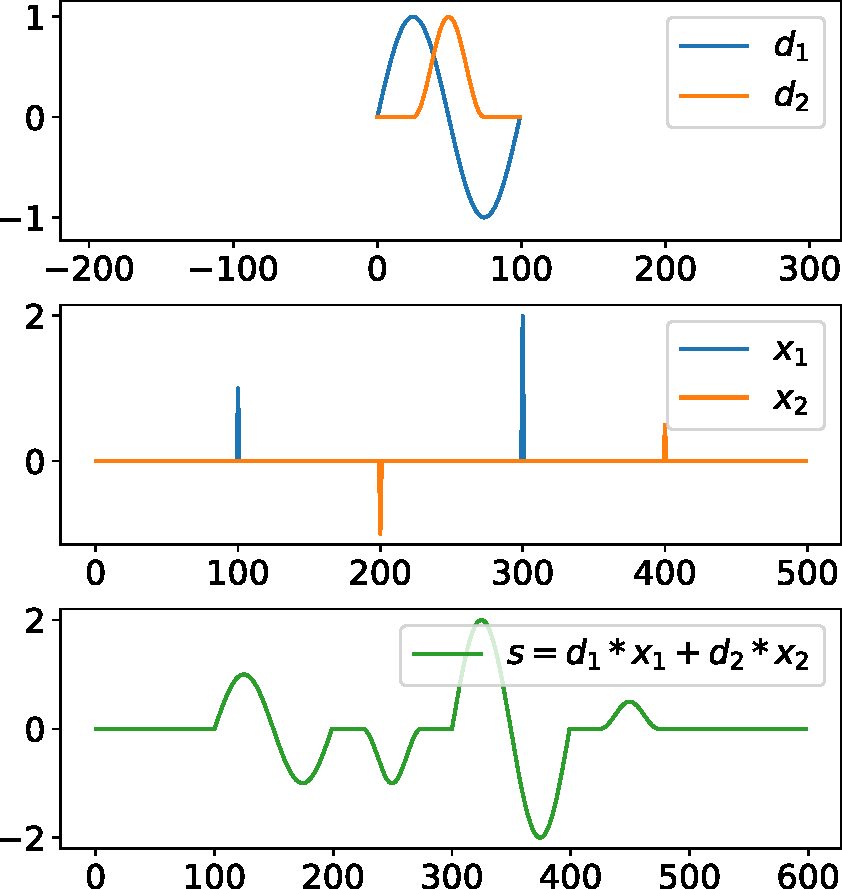
\includegraphics[width=0.9\linewidth]{cdl_example_2.pdf}\\
        \caption{Convolutional dictionary learning.}
        \label{fig:walk_class_ex_stepboxes}
    \end{figure}
\end{minipage}

\end{frame}

\begin{frame}{Signal embedding}{Learning step atoms}

\renewcommand{\ratio}{0.9}
\centering
\begin{minipage}[t]{0.45\linewidth}
\begin{itemize}
    \item Learning with Alternating Direction Method of Multipliers (ADMM) \cite{bristow2013fast}
%     \begin{itemize}
        \item 3 atoms of length 0.7 second
%     \end{itemize}

    \pause[3]
    \item Use the following embedding:
\begin{equation*}\label{eq: convolutional embedding}
\bfS \doteq \Big( \bfs * \bfd_m\Big)_{1 \le m \le 3 }
\end{equation*}
        
\end{itemize}

    \centering
    \begin{figure}
    \onslide<1->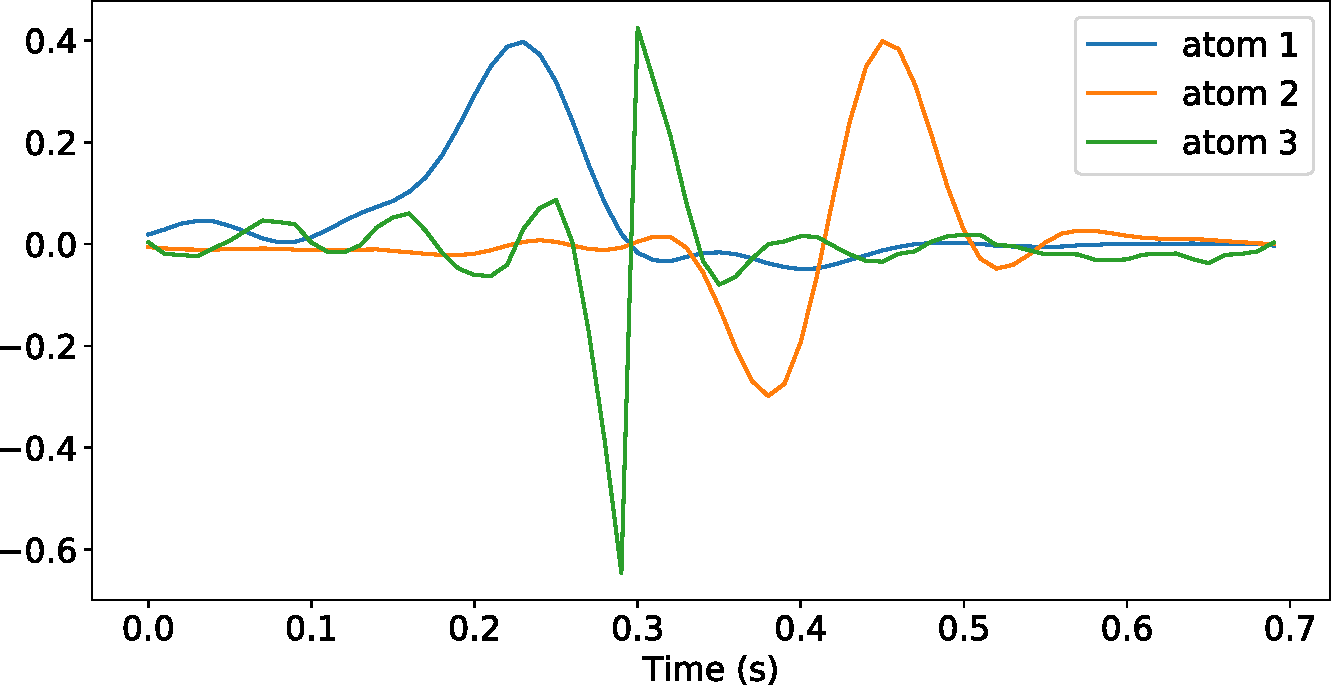
\includegraphics[width=0.85\linewidth]{dictionary.pdf}
%     \caption{Dictionary.
%         Note that the amplitude of the atoms is small compared to the signal due to the fact that they are normalized in the training process.}
    \caption{Dictionary.}
    \end{figure}
\end{minipage}
\begin{minipage}[t]{0.54\linewidth}
    \pause
    \begin{figure}
        \begin{minipage}{\linewidth}
            \centering
            \onslide<2->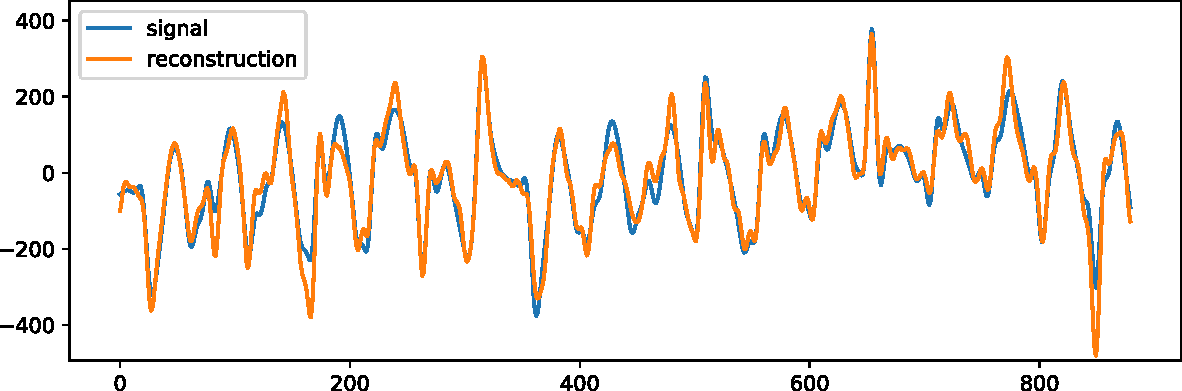
\includegraphics[trim= 0 0 0 0, width=\ratio\linewidth, clip]{signal_walk_young_female_csc_1.pdf}\\
            {\small (a)\; Original signal and its reconstruction}
        \end{minipage}\\
        \begin{minipage}{\linewidth}
            \centering
            \onslide<2->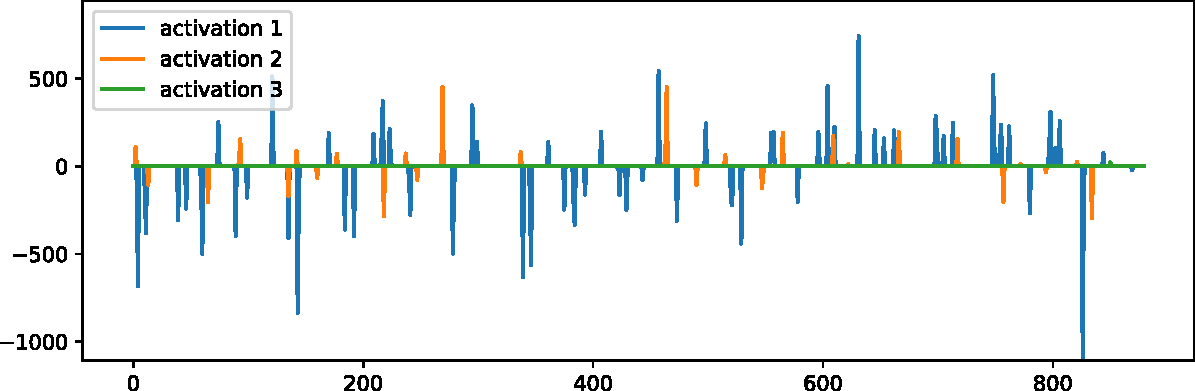
\includegraphics[trim= 0 0 0 0, width=\ratio\linewidth, clip]{signal_walk_young_female_csc_2.pdf}\\
            {\small (b)\; Signal activations}
        \end{minipage}\\
        \begin{minipage}{\linewidth}
            \centering
            \onslide<3->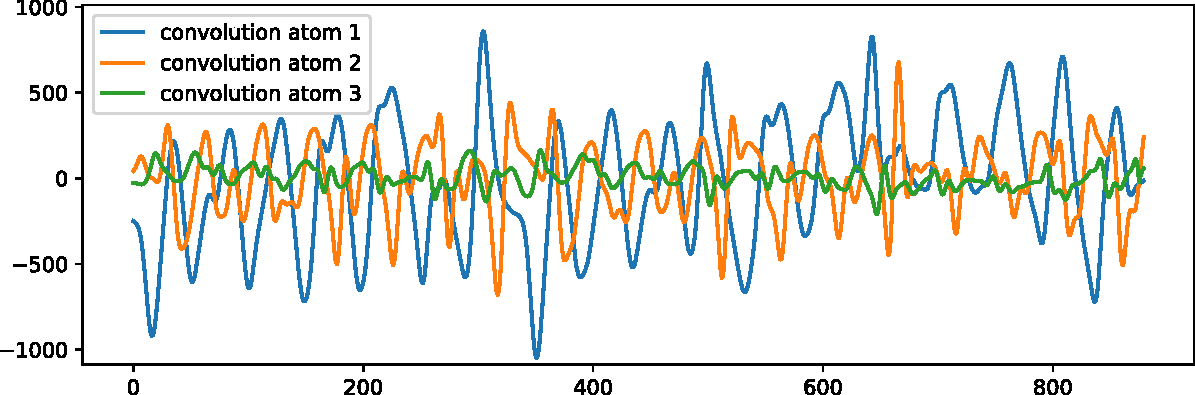
\includegraphics[trim= 0 0 0 0, width=\ratio\linewidth, clip]{signal_walk_young_female_csc_3.pdf}\\
            {\small (c)\; Embedding}
        \end{minipage}
        \onslide<2->\caption{Signal encoding and embedding.}
    \end{figure}
\end{minipage}

\end{frame}



\subsection{Step proposal network}

\begin{frame}[noframenumbering]{\ }
\hfill
\parbox[t]{.85\textwidth}{
%   \large
  \begin{minipage}[c][0.65\textheight]{\textwidth}
  \tableofcontents[currentsection, subsectionstyle=show/shaded/shaded]
  \end{minipage}
}
\end{frame}


\begin{frame}{Step proposal network}{Principle}

\begin{minipage}{0.7\linewidth}
    \begin{itemize}
        \item Objective of \subalgo: output boxes with largest Intersection over Union ($\iou$)
        \item $\iou$: $\mathbf{b_j}$ are labelled boxes, $\hat{b}$ is an estimated box:
    \begin{equation*}\label{eq: def IOU}
    \iou(\hat{b}) \doteq \max_{j} \frac{ \vert \mathbf{b_j} \cap \hat{b}\vert}{\vert \mathbf{b_j} \cup \hat{b}\vert}
    \end{equation*}
    \end{itemize}
\end{minipage}\hfill
\begin{minipage}{0.3\linewidth}
    \centering
    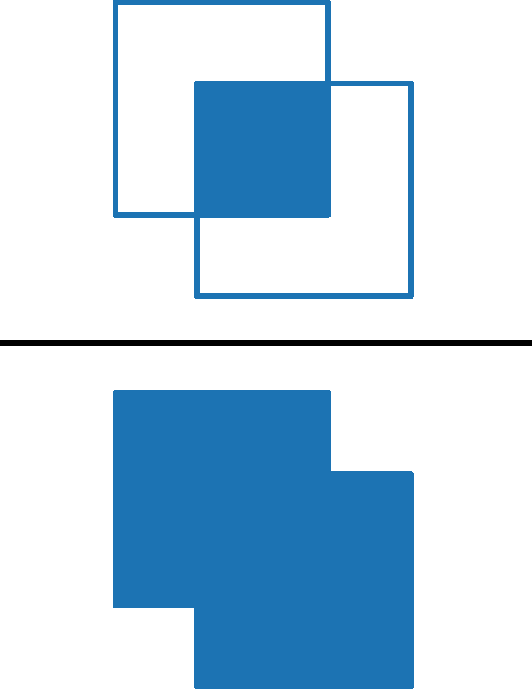
\includegraphics[width=0.7\linewidth]{iou_scheme.pdf}
\end{minipage}

\pause

\begin{figure}[h]
    \centering
    \begin{minipage}[t]{0.45\linewidth}
        \centering
        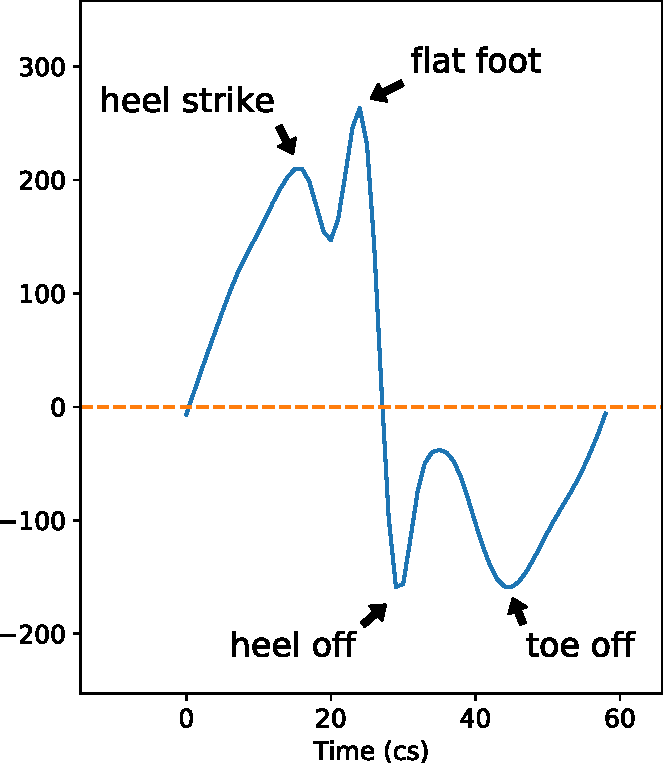
\includegraphics[width=0.6\linewidth]{example_step.pdf}\\
        {\small (a)\; Step signal}
    \end{minipage}\hfill
    \begin{minipage}[t]{0.55\linewidth}
        \centering
        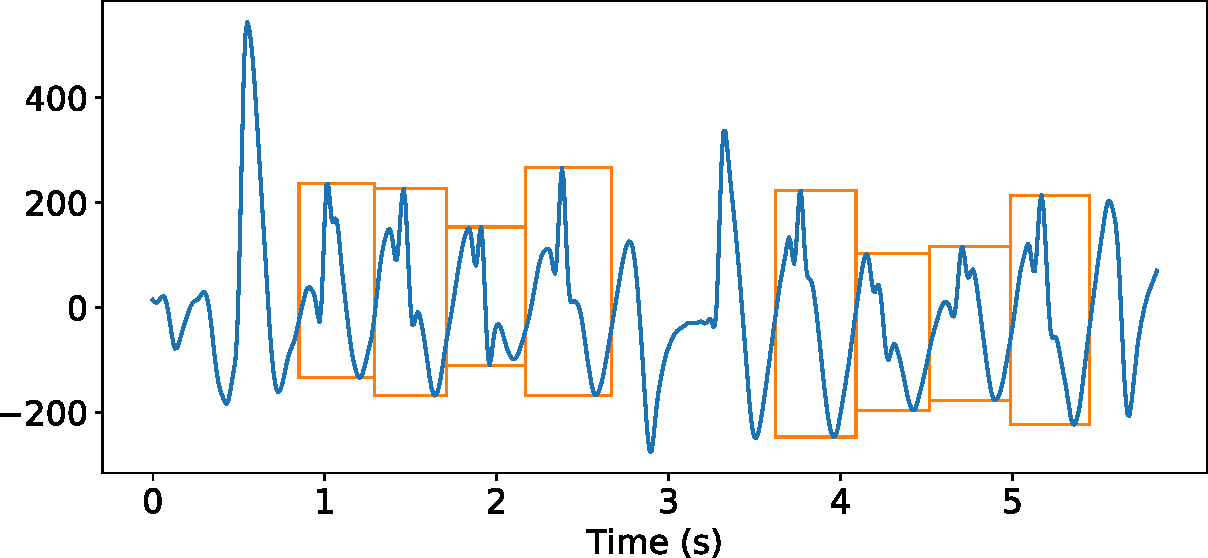
\includegraphics[width=\linewidth]{signal_walk_young_female_stepboxes.pdf}\\
        {\small (b)\; Step labels over a walk signal}
    \end{minipage}
    \caption{Example of a typical step (a) and true steps delimiting boxes in a walk signal (b).}
    \label{fig:walk_class_ex_stepboxes}
\end{figure}
\end{frame}

\begin{frame}{Step proposal network}{Training}
\begin{itemize}
    \item Output: a matrix $\mathbf{W} \in \mathbb{R}^{T \times K}$
    \begin{itemize}
        \item $T$: signal length
        \item $K$: number of different box sizes
    \end{itemize}

    \item $\mathbf{W}_{t,k}$: probability that the box $b_t^k$ starting at time $t$ and of size $0.4$s, $0.5$s, or $0.6$s (for respectively $k=1$, $2$, or $3$) has a large $\iou$ score
    \item Positive boxes: $\iou(b_t^{k}) > \sqrt{0.7}$
    \item Negative boxes: $\iou(b_t^{k}) < \sqrt{0.3}$
    \item Other are not used for training
\end{itemize}

\vspace{0.8cm}

The loss function $\mathcal{L}$ over a signal $\bfs$ is defined as:
\begin{equation*}\label{eq: loss training CNN}
\mathcal{L}(\bfs, \mathbf{W}) = \sum_{t} \sum_{k \in \left[1, 2, 3 \right]} \bbmind_{ \iou(b_t^{k})> \sqrt{0.7} } \log(\mathbf{W}_{t,k}) + \bbmind_{ \iou(b_t^{k})< \sqrt{0.3} } \log(1-\mathbf{W}_{t,k}). 
\end{equation*}
\end{frame}

\subsection{Results}

\begin{frame}[noframenumbering]{\ }
\hfill
\parbox[t]{.85\textwidth}{
%   \large
  \begin{minipage}[c][0.65\textheight]{\textwidth}
  \tableofcontents[currentsection, subsectionstyle=show/shaded/shaded]
  \end{minipage}
}
\end{frame}


\begin{frame}{Results}
\begin{minipage}[t]{0.45\linewidth}
    Data
    \begin{itemize}
        \item 43 signals recorded in a nursing home
        \item Manually labeled steps
    \end{itemize}
    Training
    \begin{itemize}
        \item \subalgo is trained using classical gradient descent
        \item Training time: < 5 minutes
        \item Inference (detection over a 10s signal): < 1 second
        \item Optimization details
        \begin{itemize}
            \item learning rate of $10^{-3}$
            \item learning rate decay ($\times 0.9$ every 10 epochs)
            \item Nesterov momentum
        \end{itemize}
    \end{itemize}
\end{minipage}\hfill
\begin{minipage}[t]{0.5\linewidth}
    \begin{figure}[h]
    %     \begin{minipage}{\linewidth}
            \centering
            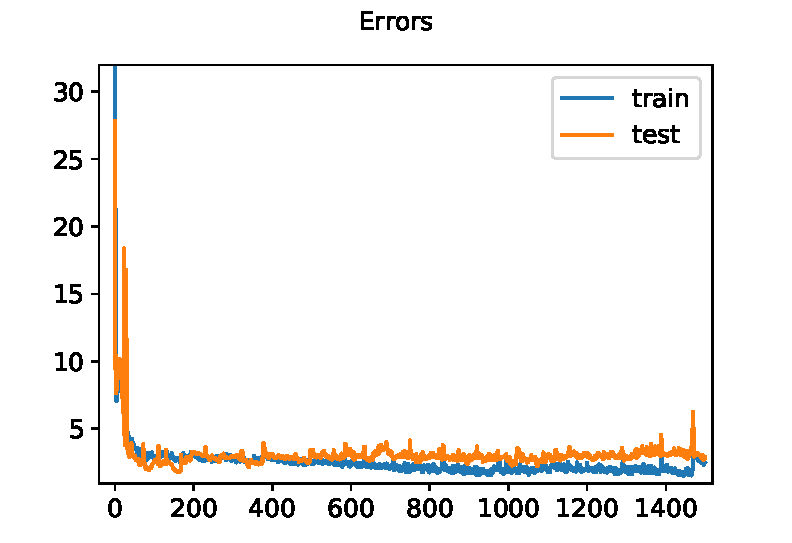
\includegraphics[width=\linewidth]{spn_train_test_errors.pdf}
    %     \end{minipage}
        \caption{\subalgo training and testing errors.}
    %     \label{fig:walk_class_spn_detection_test_example}
    \end{figure}
\end{minipage}
\end{frame}

% \begin{frame}{Results}
% \begin{figure}[h]
%     \begin{minipage}{\linewidth}
%         \centering
%         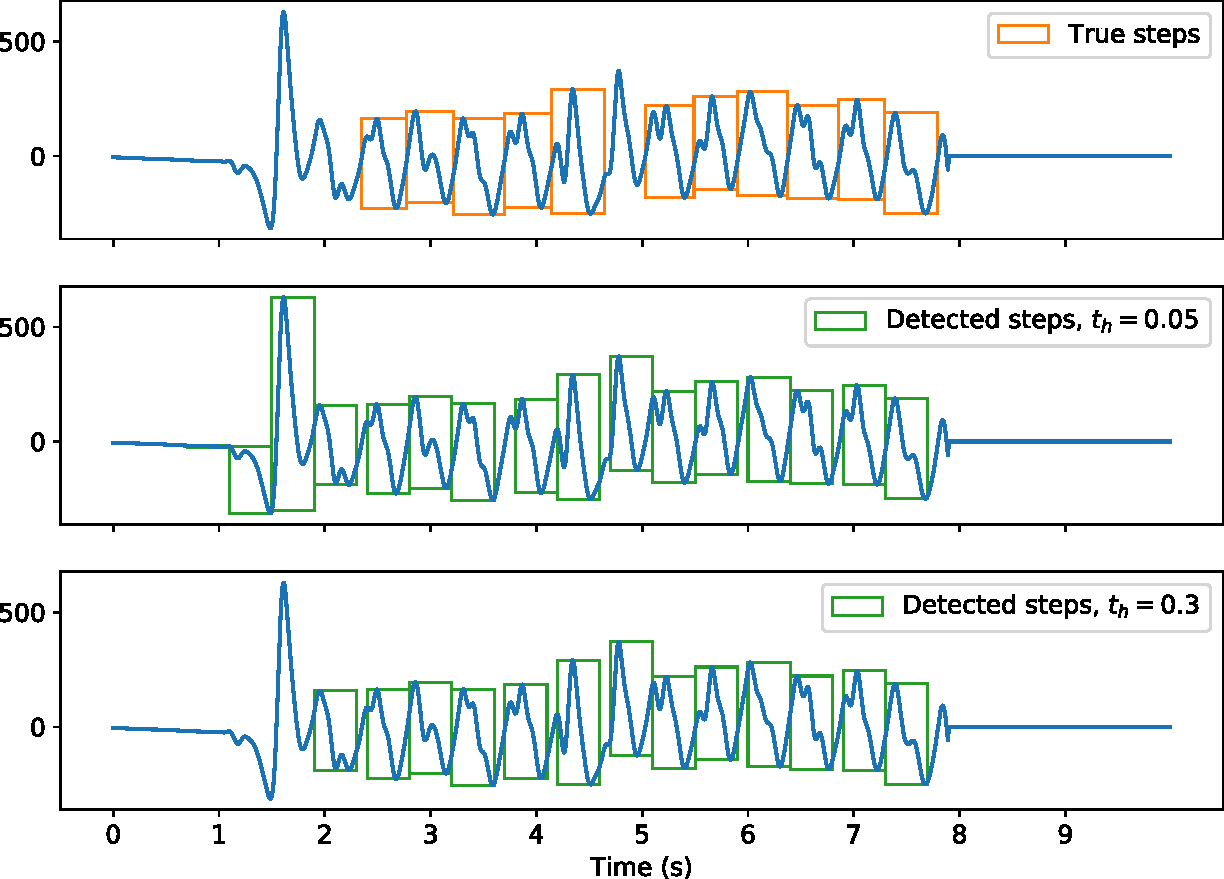
\includegraphics[width=0.75\linewidth]{SPN_Mercredi_11_28_01_00_to_11_28_08_90.pdf}
%     \end{minipage}
%     \caption{Test of \subalgo over a walk signal.}
%     \label{fig:walk_class_spn_detection_test_example}
% \end{figure}
% \end{frame}

\begin{frame}{Results}
% \animategraphics[loop,controls,width=\linewidth]{2}{Mercredi_10_19_13_00_to_10_19_18_85_th_}{1}{4}
% \animategraphics[loop,controls,width=\linewidth]{2}{test_}{1}{4}
\begin{itemize}
    \item Object detection use the mean Average Precision (mAP): area under the Precision-Recall curve
    \item \textbf{Without} embedding, mAP = 72,5\%
    \item \textbf{With} embedding, mAP = 78,6\%
\end{itemize}
\pause

\begin{figure}[h]
    \begin{overprint}
        \onslide<2>\centering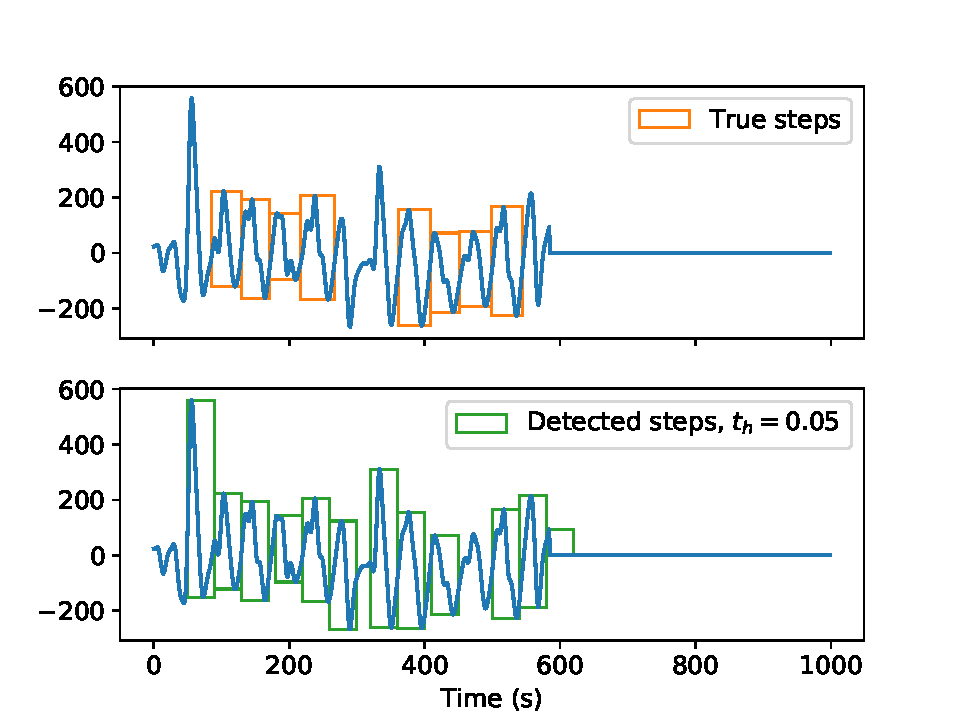
\includegraphics[width=0.75\linewidth]{Mercredi_10_19_13_00_to_10_19_18_85_th_005.pdf}
        \onslide<3>\centering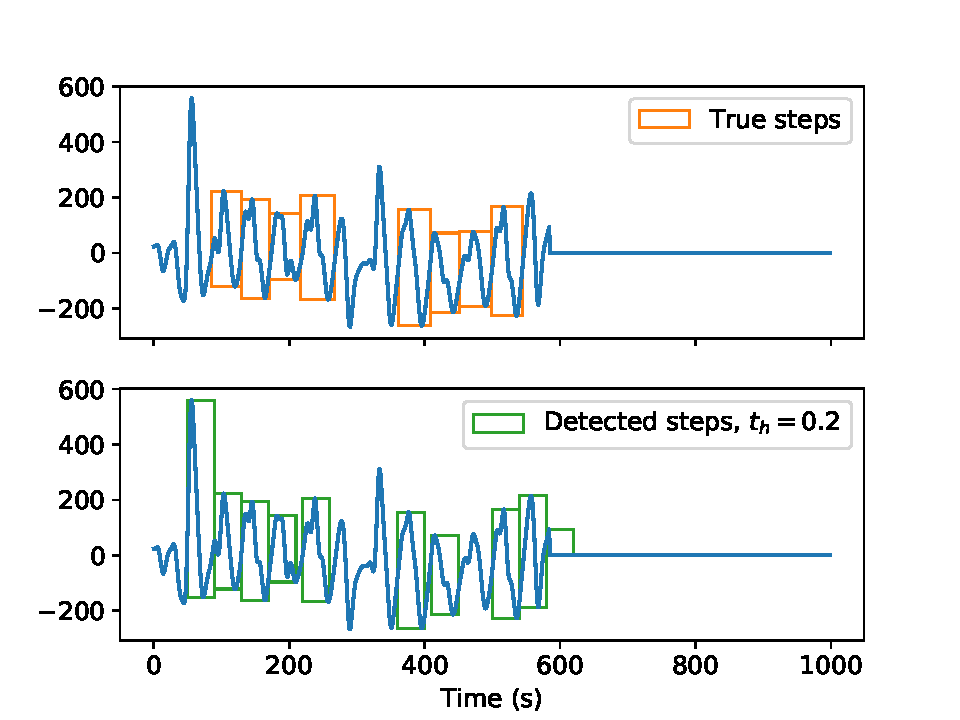
\includegraphics[width=0.75\linewidth]{Mercredi_10_19_13_00_to_10_19_18_85_th_02.pdf}
        \onslide<4>\centering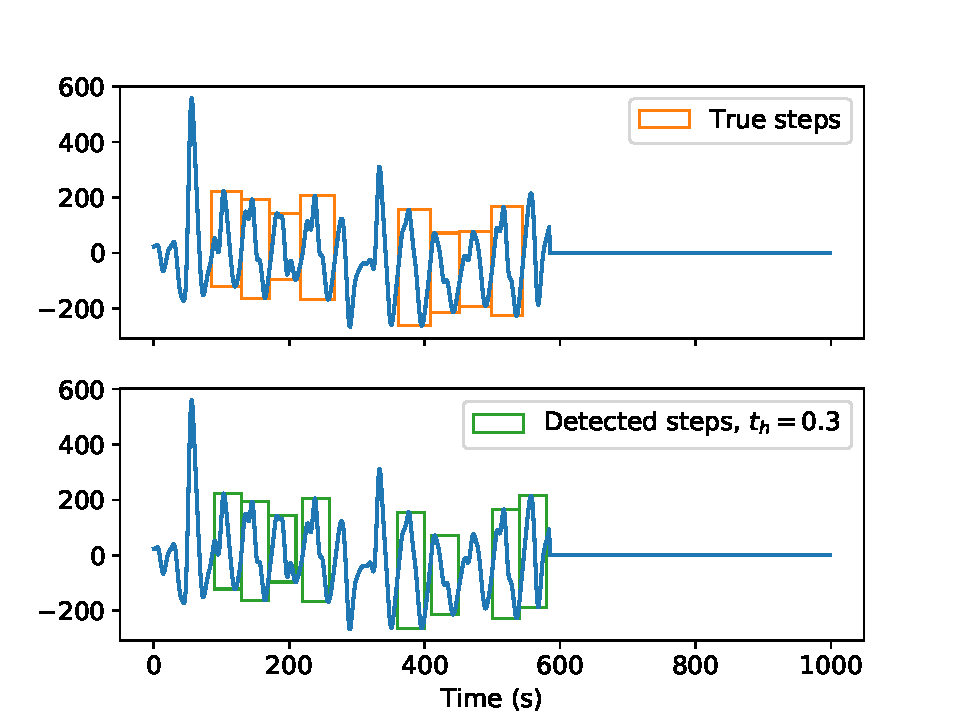
\includegraphics[width=0.75\linewidth]{Mercredi_10_19_13_00_to_10_19_18_85_th_03.pdf}
    \end{overprint}
    \caption{Test of \subalgo over a walk signal.}
\end{figure}
\end{frame}

\section{Conclusion}

\begin{frame}{Conclusion}

% \vspace{1cm}
\centering
\begin{minipage}[t]{0.8\linewidth}
Conclusion
\begin{itemize}
    \item SPN uses the convolutional representation to detect steps
    \item Allows to located steps in complex signals
    \item Training and inference are fast
\end{itemize}
Future work
\begin{itemize}
    \item Add a regression layer on the step proposals
    \item Tests on step detection benchmarks data sets
\end{itemize}
\end{minipage}

\vfill
\pause
% \vspace{1cm}
\begin{block}{\centering Thanks}
\medskip
Contact: minvielle@cmla.ens-cachan.fr\\[5pt]
Reference: L. Minvielle and J. Audiffren. Nursenet : Monitoring elderly levels of activity with a
piezoelectric floor. Sensors, 19(18), 2019
\; \href{https://www.mdpi.com/1424-8220/19/18/3851}{{\usebeamercolor[fg]{structure} link}}
\end{block}
\end{frame}

%
% ---------------------------------------------------------------
% \section{Thanks}
% \begin{frame}{Thanks}
% \end{frame}

\begin{frame}[allowframebreaks]
        \frametitle{References}
        \bibliographystyle{apalike}
        \bibliography{biblio.bib}
\end{frame}

\end{document}